\documentclass[journal=cic,version=preprint]{iacrj}

\usepackage{booktabs}
\usepackage{amssymb}

\license{CC-BY-4.0}

\title[running={SD-BKZ on NTRU}]{Self-Dual BKZ on NTRU: Dimension-Onset, Fatigue, and a Cross-Engine Reference-Free DSD Observable}

\addauthor[surname = {Chambers-Bourgeois},
           email   = {brendanchambersbou@gmail.com},
           orcid   = {0009-0004-2609-0822},
           inst    = {1}
          ]{Brendan Chambers-Bourgeois}

\addaffiliation[country={Australia},
                city={Melbourne}]{Independent Researcher}

\keywords{lattice reduction, BKZ, SD-BKZ, NTRU, overstretched, fatigue, dense sublattice discovery, Rankin profile, sieving, G6K}

\emergencystretch=3em

\begin{document}
\maketitle

\begin{abstract}
The Root Hermite Factor (RHF) is the standard one-number summary of
lattice-reduction quality; the companion paper found BKZ and self-dual BKZ
(SD-BKZ) RHF-equal on LWE-Kannan lattices yet different in Rankin profile.
This report asks whether the variants also differ on \emph{NTRU} near the fatigue point. First, the
SD-BKZ advantage on circulant NTRU is not smooth in dimension: tied with BKZ
for $n\!\le\!67$, it spikes at $n\!\approx\!71$--$73$ (mean $d(\mathrm{LN})$
advantage up to $+9.7$ nats at $q=97$, where the dense-sublattice discovery (DSD) flag cannot fire, $q<q^\ast\approx156$--$160$), then settles to a $+1.5$--$1.7$-nat plateau for $n=79$--$89$. Second,
in the overstretched $q$-onset regime the defensible observable is
\emph{reference-free}: there the signed $d(\mathrm{LN})$ is a reference
artefact. Under this observable, flag-scored at $\beta=20$, BKZ's DSD onset
sits $19\%$ above SD-BKZ's in $q$ at $n=89$ and $101$ and $28\%$ at
$n=113$ ($n\!\le\!79$ unscorable). Third, at $\beta=40$ the G6K sieve matches fplll: a gap under
$0.5\%$ at $n=89$, $6$--$9\%$ at $n=101$--$113$ on both, each engine's SD-BKZ
firing on a near-superset of BKZ's. The
engines differ in the sub-fatigue tail: under SD-BKZ at $n=89$, $q=137$ the sieve
clears it on $61/100$ seeds, enumeration on $38/100$. Fourth, at $n=157$--$185$,
scored by exact key recovery, the $\beta=40$ wall moves with
blocksize and tours in preliminary cells, and SD-BKZ leads per seed but not
per core-hour on fplll. The threat model is an adversary free to pick SD-BKZ
over BKZ at fixed blocksize and tours; no deployed parameter set is evaluated.
All experiments are reproducible via a containerised, determinism-gated
benchmark.
\end{abstract}

\paragraph{Key terms.}
\begin{description}
\setlength{\itemsep}{0pt}
\item[\textnormal{\emph{NTRU lattice}}] a structured lattice hiding a short secret key $(f,g)$.
\item[\textnormal{\emph{BKZ / SD-BKZ}}] block-reduction algorithms; SD-BKZ also reduces from the dual end each tour.
\item[\textnormal{\emph{Fatigue point}}] the modulus $q$ where reduction flips from solving SVP to finding the dense sublattice.
\item[\textnormal{\emph{DSD}}] dense-sublattice discovery---the reduced profile collapsing onto the secret sublattice.
\item[\textnormal{\emph{RHF}}] Root Hermite Factor: the usual one-number reduction-quality score.
\item[\textnormal{\emph{fplll / G6K}}] the two reduction engines: exact enumeration vs.\ randomised sieving.
\end{description}

\section{Introduction}
\label{sec:intro}

NTRU lattices fail differently from random ones. Past the fatigue
point~\cite{DucasWoerden2021}, reduction stops grinding toward a shortest
vector and discovers the dense secret sublattice wholesale. Where that
transition sits, and which algorithm crosses it first, is a question security
estimation answers with models scored by the Root Hermite Factor (RHF). The
companion paper~\cite{Paper1} found BKZ and self-dual
BKZ~\cite{EC:MicWal16} RHF-equal on LWE-Kannan lattices yet different in the
Li--Nguyen Rankin profile distance $d(\mathrm{LN})$~\cite{EPRINT:LiNgu20}. This report asks two
questions: \emph{(i) does the SD-BKZ phenomenology generalise from LWE to
NTRU?} and \emph{(ii) does it reproduce on a sieving oracle (G6K) rather than
enumeration?} Both answers are yes, with two qualifications: on NTRU only a
reference-free observable sees the difference, and at $\beta=40$, on both
engines, only from $n=101$.

Contributions:
\begin{itemize}
  \item The SD-BKZ advantage on circulant NTRU~\cite{DucasWoerden2021} has a sharp dimension-onset (Section~\ref{sec:dimonset}).
  \item A reference-free, flag-scored \emph{DSD onset} whose SD-vs-BKZ gap is $19$--$28\%$ at $\beta=20$, $n=89$--$113$ (Section~\ref{sec:fatigue}).
  \item G6K as a second engine with a validated self-dual pump-and-jump; RHF-equality holds on both engines where $\mathbf b_1$ stays a $q$-vector, as under approximate oracles~\cite{ABLR21,Rowell2024} (Section~\ref{sec:xengine}).
  \item Preliminary recovery-scored ladders at $n=157$--$185$: the $\beta=40$, $50$-tour wall moves with blocksize and tours; SD-BKZ leads per seed, not per core-hour on fplll (Section~\ref{sec:frontier}).
  \item A DSD-criterion audit: the $b_1$-only test over-fires below fatigue and manufactured a cross-engine gap (Section~\ref{sec:xengine}).
  \item The companion paper's $-345$ floors traced to our double-precision measurement GSO, not fplll, on LWE and NTRU, and that paper's wrong statements corrected (Appendices~\ref{sec:p1corr} and~\ref{sec:kahan}).
\end{itemize}

This is a \emph{technical report / data paper}: apparatus, data and
reproducibility, not new theory. Closest prior work is Deng and
Jia~\cite{DengJia2023}, whose self-dual BKZ replaces enumeration with a G6K
Pump oracle at comparable quality and lower running time, with the SD-vs-BKZ
gap narrowing as the block size grows. They do not study NTRU or DSD, and call
Pump per window inside the self-dual skeleton, where we run a full
pump-and-jump tour followed by a dual tour.
White~\cite{White26} reviews the Li--Nguyen dynamic-analysis framework and
identifies dual-lattice BKZ as a direction for it, pursued empirically here.

\section{Background}
\label{sec:background}

\subsection{Circulant NTRU lattices and fatigue}
\label{sec:bg-ntru}
We use the circulant NTRU construction of Ducas and van
Woerden~\cite{DucasWoerden2021}. For a prime $n$ and modulus $q$, sample
ternary secrets $f,g\in\mathbb{Z}_q[x]/(x^n-1)$ (uniform $\{-1,0,1\}$,
coordinate variance $\sigma^2=2/3$) with $f$ invertible, set $h=g/f \bmod q$,
and form the $2n\times2n$ basis
\[
B=\begin{pmatrix} q I_n & 0 \\ H & I_n \end{pmatrix},
\]
where $H$ is the circulant matrix of $h$. The secret $(f,g)$ is an unusually
short vector in the row span. Two structures distinguish $B$ from a random
lattice: a \emph{$q$-vector head} (rows of $qI_n$ surviving reduction at length
$q$) and a \emph{dense secret sublattice} spanned by the rotations of $(f,g)$.
A BKZ-reduced NTRU profile therefore follows the Z-shaped \emph{ZGSA} of
Ducas and van Woerden~\cite{DucasWoerden2021}: a flat head at $\log q$, a GSA
slope, and a flat tail at $0$, until DSD breaks it. The same shape is studied
for $q$-ary SIS~\cite{DEP2023}.

As $q$ grows at fixed $n$, the secret sublattice becomes relatively denser: at
the \emph{fatigue point}
$q_\mathrm{fat}(n)\approx0.004\,n^{2.484}$~\cite{DucasWoerden2021} (fit for
$n>100$, extrapolated below here) reduction passes from the standard regime
(secret found only through full SVP) to the \emph{overstretched} regime, where
it discovers the dense sublattice (\emph{dense-sublattice discovery}, DSD)
before solving SVP.

\subsection{BKZ, SD-BKZ, and the two engines}
\label{sec:bg-bkz}
Block Korkine--Zolotarev (BKZ) reduction repeatedly calls an SVP oracle on
length-$\beta$ projected sublattice windows, sweeping left to right. Self-dual
BKZ (SD-BKZ)~\cite{EC:MicWal16} alternates a forward (primal) pass with a
backward pass on the reversed dual basis, so each tour reduces the basis from
both ends. On LWE-Kannan lattices the companion paper~\cite{Paper1} found the
two produce bases of indistinguishable Root Hermite Factor%
\footnote{The stored quantity is the un-rooted Hermite factor
$\|\mathbf b_1\|/\det(L)^{1/d}$; BKZ--SD-BKZ differences on the same lattice
are convention-independent.} yet measurably different Rankin profiles.

We use two engines. \textbf{fplll} supplies an exact enumeration SVP oracle
and a native self-dual variant, our ground truth. \textbf{G6K}~\cite{G6K2019}
supplies an approximate \emph{sieving} oracle through the pump-and-jump BKZ
tour; we realise SD-BKZ on it as a primal pump-and-jump pass followed by a
dual pass in G6K's dual mode.
Wang~\cite{Wang2024} bounds the tour count and Hermite factor of the
pump-and-jump tour analytically; we use it only as an oracle and make no
convergence claim. All cross-engine experiments use $\beta=40$, where G6K's
default dimensions-for-free is still zero, so the sieve runs on the full
block.

\subsection{The reference-free DSD observable}
\label{sec:bg-obs}
The companion paper's metric is $d(\mathrm{LN})=\frac1m\sum_i|r_i-\rho_i|$,
where $r_i$ is the slope-removed Gram--Schmidt log-norm profile and $\rho_i$ is
the Li--Nguyen BKZ fixed point~\cite{EPRINT:LiNgu20}---a GSA line valid for a
\emph{random $q$-ary} lattice. NTRU is not (Section~\ref{sec:bg-ntru}): its
Z-shaped profile has no closed-form Li--Nguyen fixed point, so the
\emph{signed} advantage
$d(\mathrm{LN})_{\mathrm{BKZ}}-d(\mathrm{LN})_{\mathrm{SD}}$ conflates
structure with dynamics and can flip sign under another reference---a
\emph{reference artefact}.

Two observables survive this. First, the \emph{unsigned} profile divergence
$\frac1m\sum_i|r_i^{\mathrm{BKZ}}-r_i^{\mathrm{SD}}|$ never names $\rho$
(Section~\ref{sec:fatigue}). Second, and reported throughout, a binary
\emph{dense-sublattice-discovery} flag with a \emph{two-part} criterion: the
profile has collapsed onto the secret sublattice,
$\#\{i:\log\|\mathbf b_i^\ast\| < \log\sqrt{2n\cdot2/3}+0.5\}\le n+1$,
\emph{and} the shortest GS vector clears the floor,
$b_1=\min_i\log\|\mathbf b_i^\ast\| > 1.5$. The count threshold is the
$q$-independent ternary-secret log-norm plus a $0.5$-nat margin, evaluated per
$n$ ($2.75$ at $n=67$ to $3.01$ at $n=113$; Section~\ref{sec:fatigue} tests
freezing it). At $n=89$ the log-norm is $2.39$, above the $q$-independent
$b_1$ saturation ${\approx}1.96$ at full DSD (G6K, $\beta=40$, seeds 1--20
at each $q\in\{211,\dots,521\}$: SD $1.959$ / BKZ $1.956$). The
onset $q$ is where the per-seed DSD rate crosses $50\%$, interpolated linearly
between adjacent $q$-grid cells; the SD-vs-BKZ onset \emph{gap} is the object
of Sections~\ref{sec:fatigue} and~\ref{sec:xengine}, and
Section~\ref{sec:xengine} shows why the $b_1$ half alone is not a DSD flag.

\emph{Range of validity.} The scored cells ($n\le113$) predate the
integer-exact recovery field \texttt{secret\_recovered}, so the two-part flag
is the sole DSD verdict there, unvalidated against recovery. Where both
verdicts exist below the frontier---two of the seven auxiliary $\beta=40$
ladders excluded from the totals of Table~\ref{tab:coverage}, at
$n=109$ ($q\in[503,929]$) and $n=127$ ($q\in[743,1361]$), 20 seeds per
cell---the flag agrees with recovery on $317/320$
legs with no false fire; the three misses are BKZ recoveries at $n=127$, two
with $b_1\le1.5$ and one with more than $n{+}1$ short vectors; at $q=947$ the
flag alone would read SD $20$ vs BKZ $18$ where recovery is $20/20$ on both.
Five further ladders at $n\in\{131,137,139,149,151\}$
($1{,}120$ legs, $1.08$--$2.01\times q_\mathrm{fat}$) show that miss mode
growing with $n$, from $6/121$ to $21/37$ legs, again without a false fire.
The flag does not transfer to the frontier: over every canonical $50$-tour fplll
$\beta=40$ cell at $n\in[157,181]$ ($3{,}360$ legs; Section~\ref{sec:frontier})
the count half passes on every leg, so the verdict reduces to the $b_1>1.5$
floor, which only $20$ legs clear (all at $n=157$).
\texttt{secret\_recovered} marks a reduced-basis row whose exact integer norm
is no longer than the planted secret's; computed from the integer basis, it is
immune to the measurement floor of Appendix~\ref{sec:kahan}. It over-counts:
whenever $g(1)=0$ (roughly $4\%$ of keys at these $n$) we have $h(1)\equiv0
\pmod q$, so the all-ones vector $(0,\mathbf 1)$ of squared norm $n$ lies in
the key lattice and is shorter than the key ($\approx4n/3$). Every one of the
$12$ recovered-but-not-exact legs in the corpus ($11$ fplll, $1$ G6K) has
$g(1)=0$ and squared norm exactly $n$. Recovery is therefore reported as
\texttt{secret\_exact\_match}: a row equal to $\pm$ a rotation of the secret.
Against this verdict the flag is precise ($20/20$) but detects only $20$ of
$557$ fplll recoveries ($3.6\%$); the $50$-tour G6K $\beta=40$ cells at
$n\in\{167,173,179\}$ ($480$ legs) add $15$ undetected recoveries and no fire
(pooled $20/572$, $3.5\%$).

\section{Experimental Setup}
\label{sec:setup}

\subsection{Generators and engines}
\label{sec:setup-engines}
NTRU bases follow Section~\ref{sec:bg-ntru}; each basis is checked per seed
before reduction ($\dim=2n$ and $H\!f\equiv g\pmod q$).
The G6K self-dual tour was validated
against fplll's native self-dual variant (\texttt{SD\_VARIANT}) on a random $q$-ary lattice ($n=80$,
$\beta=40$, three tours): the SD-minus-BKZ GS-slope change agrees across
engines (fplll $-0.00039$ vs G6K $-0.00040$).

\subsection{Reproducibility and determinism gates}
\label{sec:setup-repro}
Both engines run in containers built from a digest-pinned base with
pinned apt snapshots. The G6K image targets \texttt{x86-64-v2} with
native-ISA detection disabled. The $n\le113$ cells (June 2026) ran an
earlier build whose configure step appended the host's AVX2/FMA over that
target; the frontier cells (August--early October) ran the corrected build,
patched from 2 September. The AVX2 and corrected builds give the same
SHA-256 for the $n=80$, $\beta=60$ reference-probe basis and $r$-profile.
Each result is a per-seed JSON
carrying the full input parameters and output profile, and a SHA-256 seed
manifest gates byte-identity. A verify script further holds the
fplll path to numerical reproducibility ($10^{-4}$ tolerance on reference
seeds) and the G6K path to an exact SHA-256
match against a captured reference hash, confirmed on a second machine.

G6K's multi-threaded
sieve has a nondeterministic reduction race, so all sieving runs single-threaded
($\texttt{threads}=1$); across-seed parallelism still uses all cores. The
fplll global RNG must be seeded before basis construction and again before the
sieve (G6K samples from it); the \texttt{SieverParams} seed is a no-op we never
rely on. With these, multi-tour G6K runs are bit-identical run-to-run; the
construction seed determines all tours (per-tour re-seeding verified a
no-op), so we seed once at construction.

\subsection{Campaigns and parameter grids}
\label{sec:setup-campaigns}
Every experiment is a named campaign fixing
generator, engine, $n$-grid, $\beta$, $q$, tour count, and seed count, so a
single command reproduces a cell. The dimension-onset sweep
(Section~\ref{sec:dimonset}) fixes $q=97$, $\beta=20$, 50 tours and sweeps
$n\in[59,89]$ at 20 seeds each ($n=71$ at 40). The fatigue and DSD-onset sweeps
(Section~\ref{sec:fatigue}) fix $n$, $\beta=20$ and 50 fplll tours and sweep
$q$ across the fatigue point. The
cross-engine sweeps (Section~\ref{sec:xengine}) fix $n=89$, $\beta=40$, 50 tours
and sweep a matched $q$-grid on both engines. The patched-fplll $n=127$ runs
(Appendix~\ref{sec:kahan}) at $q\in\{971,1087,1201\}$, on two builds, are
separate campaigns outside the canonical seeds.
Table~\ref{tab:coverage} summarises the analysed grid over 81 distinct moduli.

\begin{table}[t]
\caption{Experimental coverage. Circulant NTRU (lattice dimension $2n$), each seed a
matched BKZ / SD-BKZ reduction, on two oracles: fplll enumeration and G6K sieve.
Default 50 tours (the $n=67$ G6K entry includes four 10-tour determinism-check
seeds at $q=97$). fpylll precision is 250 bits, except 500--1000 at $q\ge569$, 500
in eight other $n=89$ cells and in eight reruns of the $n=89$, $\beta=20$,
$q=97$ cell. Totals: 8{,}704 seed pairs over 147 $(n,\beta,q)$ cells,
$\approx$6{,}430 core-hours. The $n=127$ row lists the
$\beta=20$ cells only and also carries 12 seeds rerun on two patched-fplll
builds (48 runs, both legs; Appendix~\ref{sec:kahan}). Seven native-fplll $\beta=40$ ladders
($n\in\{109,127,131,137,139,149,151\}$, $36$ cells) are in the public seed
manifest, excluded from all totals and used only for Section~\ref{sec:bg-obs}.}
\label{tab:coverage}
\centering
\begin{tabular}{rrcccrr}
\toprule
$n$ & $2n$ & $\beta$ & \#$q$ & $q$ range & $N_{\mathrm{fplll}}$ & $N_{\mathrm{G6K}}$ \\
\midrule
59  & 118 & 20    & 1  & 97        & 20   & --   \\
61  & 122 & 20    & 1  & 97        & 20   & --   \\
67  & 134 & 20,40 & 12 & 97--193   & 340  & 24   \\
71  & 142 & 20    & 1  & 97        & 40   & --   \\
73  & 146 & 20    & 1  & 97        & 20   & --   \\
79  & 158 & 20,40 & 15 & 97--293   & 380  & 20   \\
83  & 166 & 20    & 1  & 97        & 20   & --   \\
89  & 178 & 20,40 & 31 & 97--691   & 2508 & 1580 \\
101 & 202 & 20,40 & 23 & 97--541   & 1480 & 140  \\
113 & 226 & 20,40 & 25 & 97--1279  & 1340 & 620  \\
127 & 254 & 20    & 16 & 547--1811 & 152  & --   \\
\midrule
\multicolumn{5}{r}{total} & 6320 & 2384 \\
\bottomrule
\end{tabular}
\end{table}

\section{The SD-BKZ Advantage Has a Dimension-Onset on NTRU}
\label{sec:dimonset}

On circulant NTRU at $q=97$ (standard regime throughout, only marginally so at
the smallest dimension, $q_\mathrm{fat}(59)\approx100$), the SD-BKZ advantage
over BKZ has a sharp dimension transition, not a smooth ramp:

\begin{table}[tbp]
\centering
\caption{SD-BKZ advantage on NTRU: tied $\to$ onset spike $\to$ plateau.\label{tab:dimonset}}
\begin{tabular}{rrrr}
\toprule
$n$ & mean adv & std (sample) & seeds$>0$ \\
\midrule
59--67 & $\sim 0$  & $0.02$--$0.03$ & 3--9/20 \\
71     & $+4.33$   & 5.50  & 27/40 \\
73     & $+9.68$   & 5.21  & 19/20 \\
79--89 & $+1.5$--$1.7$ & $0.20$--$0.33$ & 20/20 \\
\bottomrule
\end{tabular}
\end{table}

Three regimes (Table~\ref{tab:dimonset}; Figure~\ref{fig:dimonset}): tied for
$n\!\le\!67$; an onset zone at $n=71$--$73$ with standard deviation up to
${\approx}27\times$ the plateau's; and a stable plateau for $n=79$--$89$. The
spike exceeds the plateau: the transition is non-monotonic. The onset variance is not Gaussian
noise: at $n=71$, $15/40$ seeds stay tied ($|\mathrm{adv}|<0.25$) and $25$
diverge, $22$ positive ($+1.7$ to $+13.6$) and $3$ negative ($-2.7$ to
$-6.7$); at $n=73$,
$19$ of $20$ are positive ($+1.2$ to $+16.0$; one at $-5.1$). The two-part
DSD criterion fires on no seed of either variant at $n=71$ or $73$. One scale caveat: the NTRU $d(\mathrm{LN})$ baseline (${\approx}50$)
sits an order of magnitude above the LWE-Kannan scale (final $d(\mathrm{LN})$
${\approx}4$--$5$ at the companion paper's central cells), so only sign and
structure, not raw nats, carry across to the companion paper.

\begin{figure}[tbp]
\centering
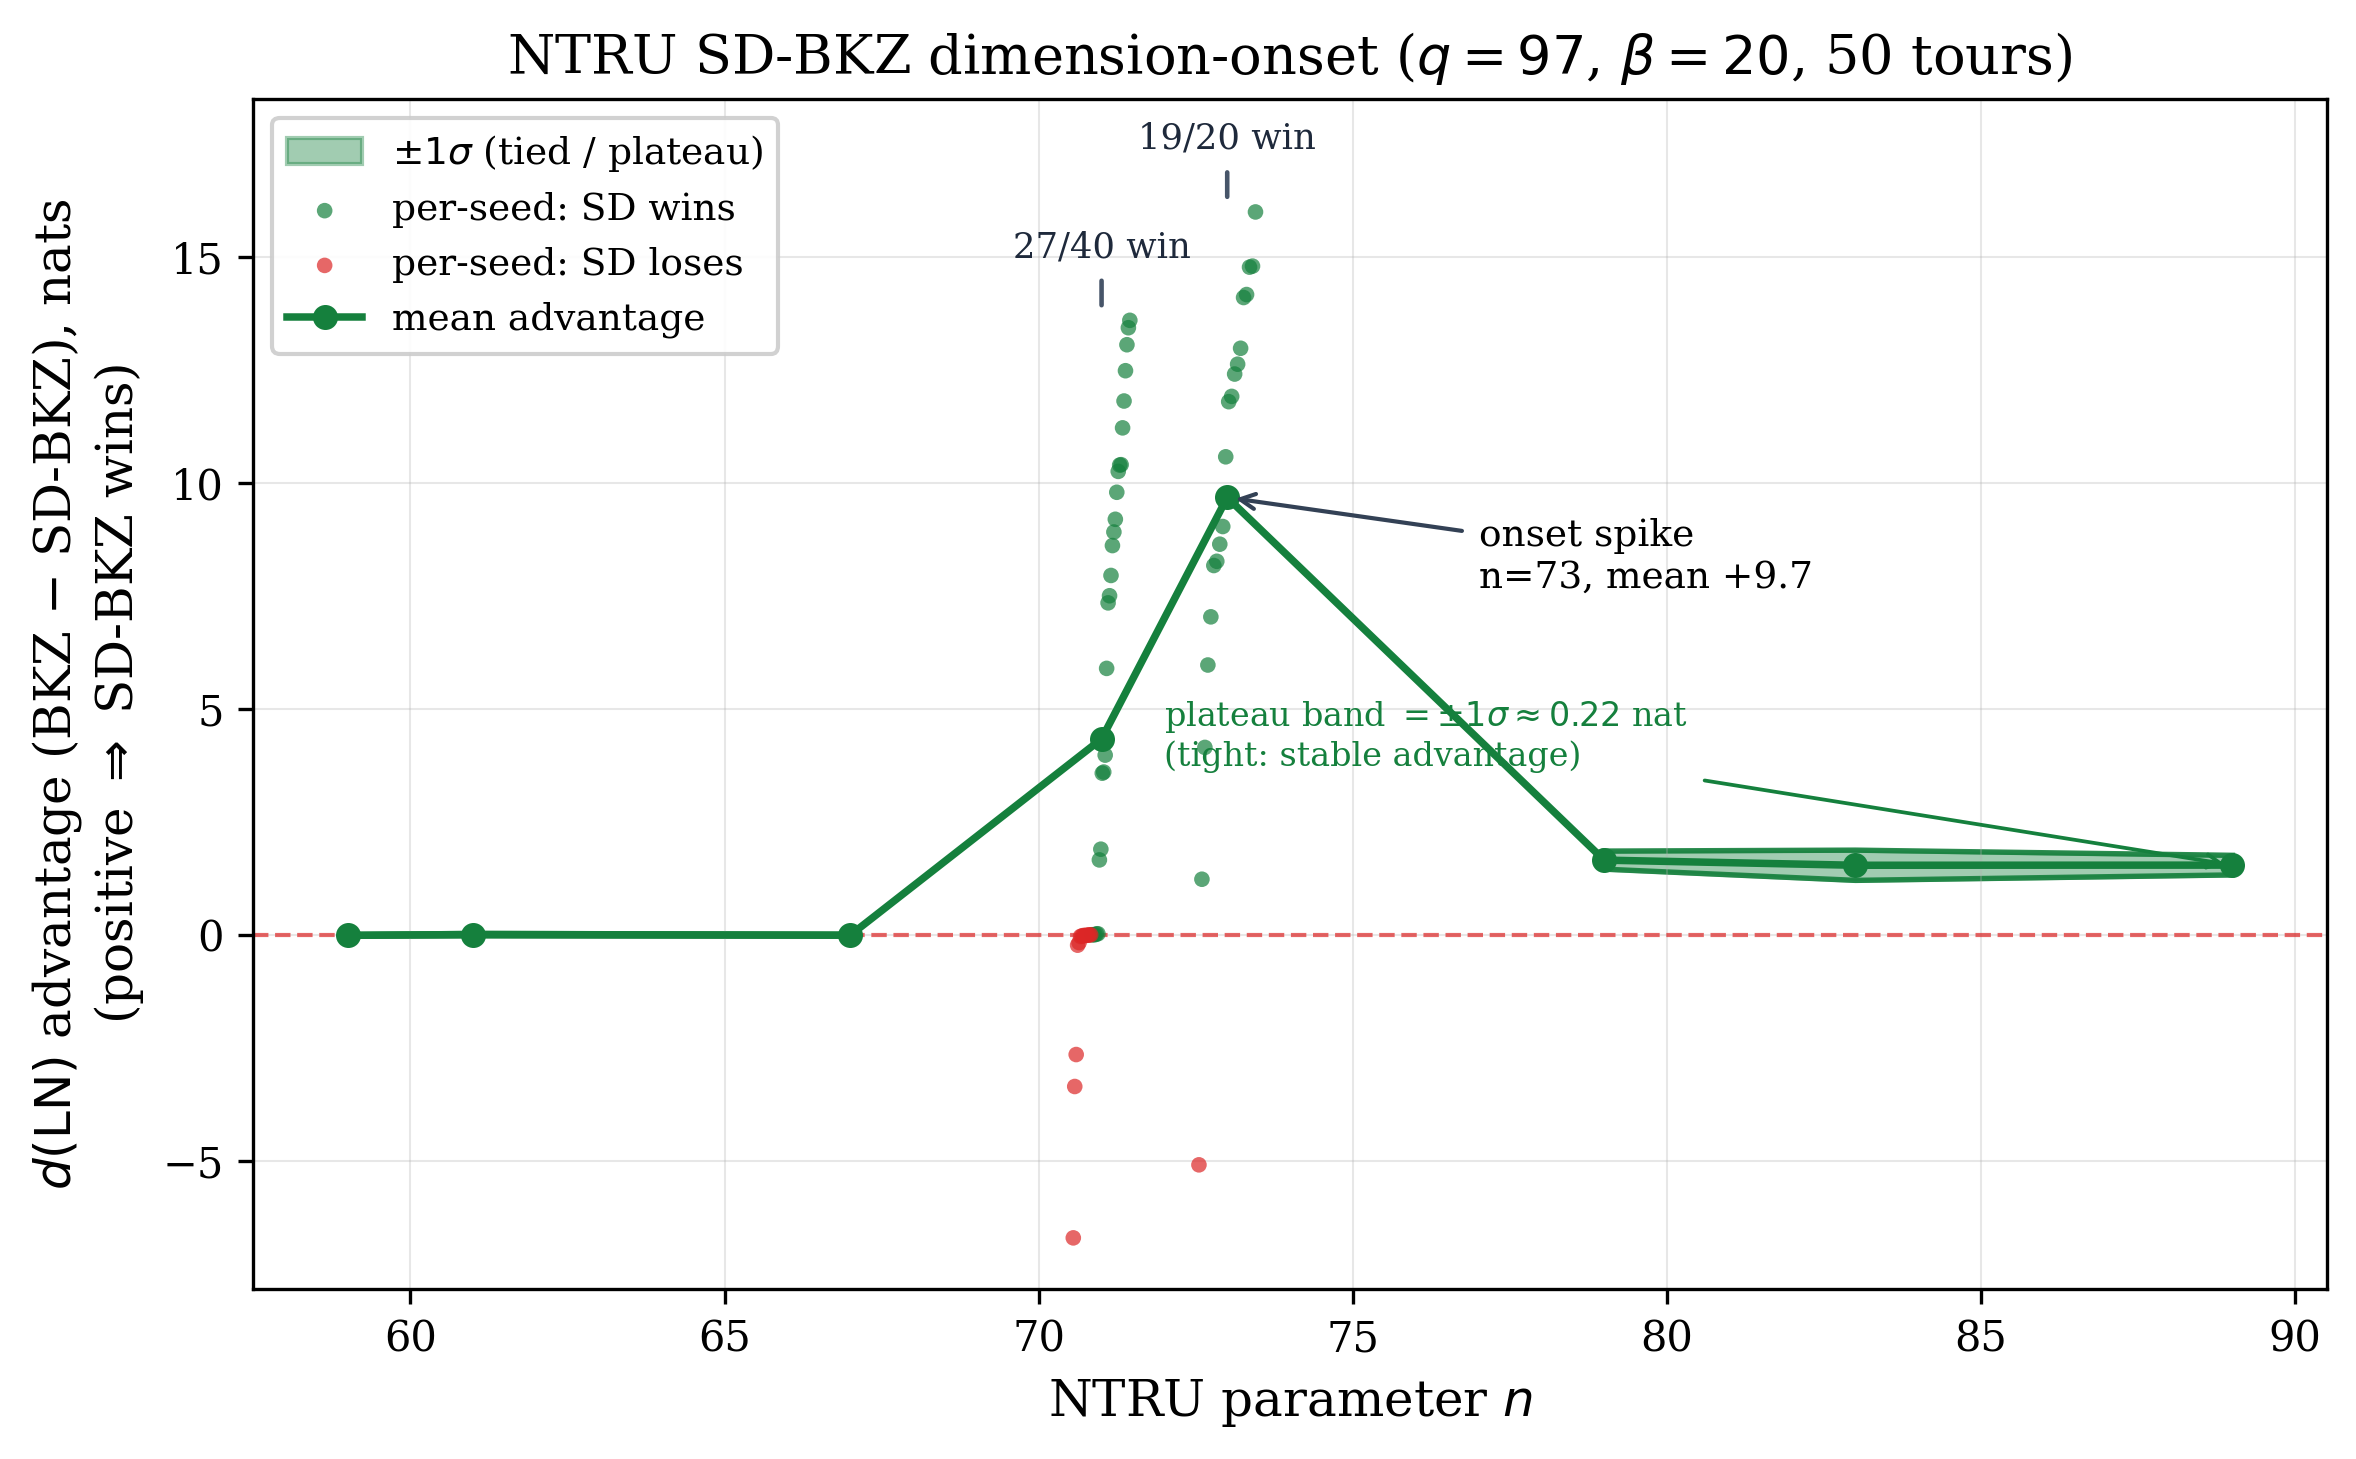
\includegraphics[width=\linewidth]{figs/dimension_onset}
\caption{NTRU SD-BKZ dimension-onset ($q=97$, $\beta=20$, 50 tours, 20 seeds
per $n$, $n=71$ at $40$; in the onset zone $n=71$--$73$ the per-seed
advantages are plotted individually and coloured by sign, since the spread
is not Gaussian; spread per regime is in
Table~\ref{tab:dimonset}). The signed advantage
is reference-robust at the spike (Section~\ref{sec:fatigue}); shown here for
the dimension transition. Recomputed from the per-seed \texttt{advantage}
field.\label{fig:dimonset}}
\end{figure}

\section{Fatigue and the Cross-Dimension DSD-Onset Gap}
\label{sec:fatigue}

The $n\approx71$--$73$ divergence of
Section~\ref{sec:dimonset} is reference-robust: re-derived from the stored
profiles under three references (Li--Nguyen, GSA-zero, and the reference-free
$\frac1m\sum_i|r_i^{\mathrm{BKZ}}-r_i^{\mathrm{SD}}|$), it stays large
($32.7$ nats reference-free at $n=73$ vs $0.03$ at $n=67$) and sign-stable
($n=73$ mean $+9.68$ under Li--Nguyen vs $+28.1$ under GSA-zero; $n=67$ $-0.01$
and $n=79$ $+1.65$ under both). In
the overstretched $q$-onset regime the signed advantage is a reference artefact
(Section~\ref{sec:bg-obs}), so the onset results below use the reference-free
DSD observable; the per-tour $d(\mathrm{LN})$ curves of
Section~\ref{sec:dynamics} serve only as timing.

At fixed $n$ the reference-free BKZ-vs-SD-BKZ profile divergence peaks
between the two variants' onsets, not at $q_\mathrm{fat}$ ($0.92$, $1.23$,
$1.54\,q_\mathrm{fat}$ at $n=89$, $101$, $113$). From $n=89$ the
SD-BKZ DSD-onset falls at \emph{lower} $q$ than BKZ's:

\begin{table}[tbp]
\centering
\caption{Reference-free DSD-onset ($\beta=20$, fplll, 50 tours; two-part criterion): SD-BKZ reaches dense-sublattice discovery at lower $q$ than BKZ for $n\ge89$. $^\ast$The $n=67$ and $79$ rows are not transitions: the criterion cannot fire below $q^\ast=(4n/3)\sqrt{e}$ ($147$, $174$), and $\mathbf b_1$ is already secret-length on every seed of both variants at every sampled $q$ at $n=67$, and on all but one from $q=157$ at $n=79$; these onsets measure the criterion and carry no SD-vs-BKZ information. Onsets are $50\%$-rate crossings, linearly interpolated between grid cells; gap\% is computed from these unrounded onsets (denominator: SD onset). Bracketing cells carry $N=100$ seeds at $n\ge89$ and $N=20$ at $n=67/79$; the $n=113$ endpoint comes from the $q$-sweep (precision $250$--$1000$ bits by $q$, Table~\ref{tab:coverage}).\label{tab:dsdgap}}
\begin{tabular}{rrrr}
\toprule
$n$ & SD onset $q$ & BKZ onset $q$ & gap\% \\
\midrule
67$^\ast$  & 144.6 & 145.4 & -- \\
79$^\ast$  & 171.2 & 171.0 & -- \\
89  & 238.0 & 283.3 & 19 \\
101 & 428.6 & 512.2 & 19 \\
113 & 729.2 & 930.4 & 28 \\
\bottomrule
\end{tabular}
\end{table}

The extraction evaluates the short-count threshold per $n$
(Section~\ref{sec:bg-obs}). Because that threshold exceeds the whole
dense-sublattice step $\log q-\log\|s\|$ whenever
$q<q^\ast=\|s\|\,e^{\mathrm{thr}(n)}=(4n/3)\sqrt e$, the count half cannot
pass below $q^\ast$ however reduced the basis is: at $n=67$ the flag goes
$0/20\to17/20$ between $q=139$ and $149$ and at $n=79$ $1/20\to14/20$
between $167$ and $173$, straddling $q^\ast$ while $\mathbf b_1$ is
secret-length throughout. At $n=89$ the onset ($238/283$) sits above
$q^\ast=196$ and the $\mathbf b_1$ rates separate the variants ($88/100$ vs
$47/100$ at $q=223$), so the $n\ge89$ rows measure the lattice. Freezing the
threshold at its $n=89$ value $2.888$ shifts only the $n\le79$ rows
($166.6/167.5$; $181.7/182.5$) and $n=113$ BKZ ($925.0$, gap $27\%$),
leaving the gap trend unchanged. $n=127$ is excluded from the $\beta=20$ trend and onset figures:
the integer-exact recovery field was not recorded for its $152$ $\beta=20$
seeds; $16$ of them carry the $-345$ floor of the double-precision
measurement GSO (Appendix~\ref{sec:kahan}); and its SD-BKZ DSD rate never reaches $50\%$ on
the sampled ladder (${\le}25\%$ up to $q=1811\approx2.7\,q_\mathrm{fat}$; BKZ
$0\%$). The $80$ $n=127$ $\beta=40$ manifest seeds, outside Table~\ref{tab:coverage}, do
carry the verdict: $1/20$ vs $1/20$ at $q=743$, $20/20$ on both legs at
$q\ge947$; the $80$ $n=109$ $\beta=40$ seeds, likewise outside the totals,
recover $20/20$ on both legs at every rung $q\in\{503,647,787,929\}$
($1.09$--$2.02\times q_\mathrm{fat}$), so that ladder starts above its onset.
Figure~\ref{fig:phase} plots the onsets against the fatigue curve.

\begin{figure}[tbp]
\centering
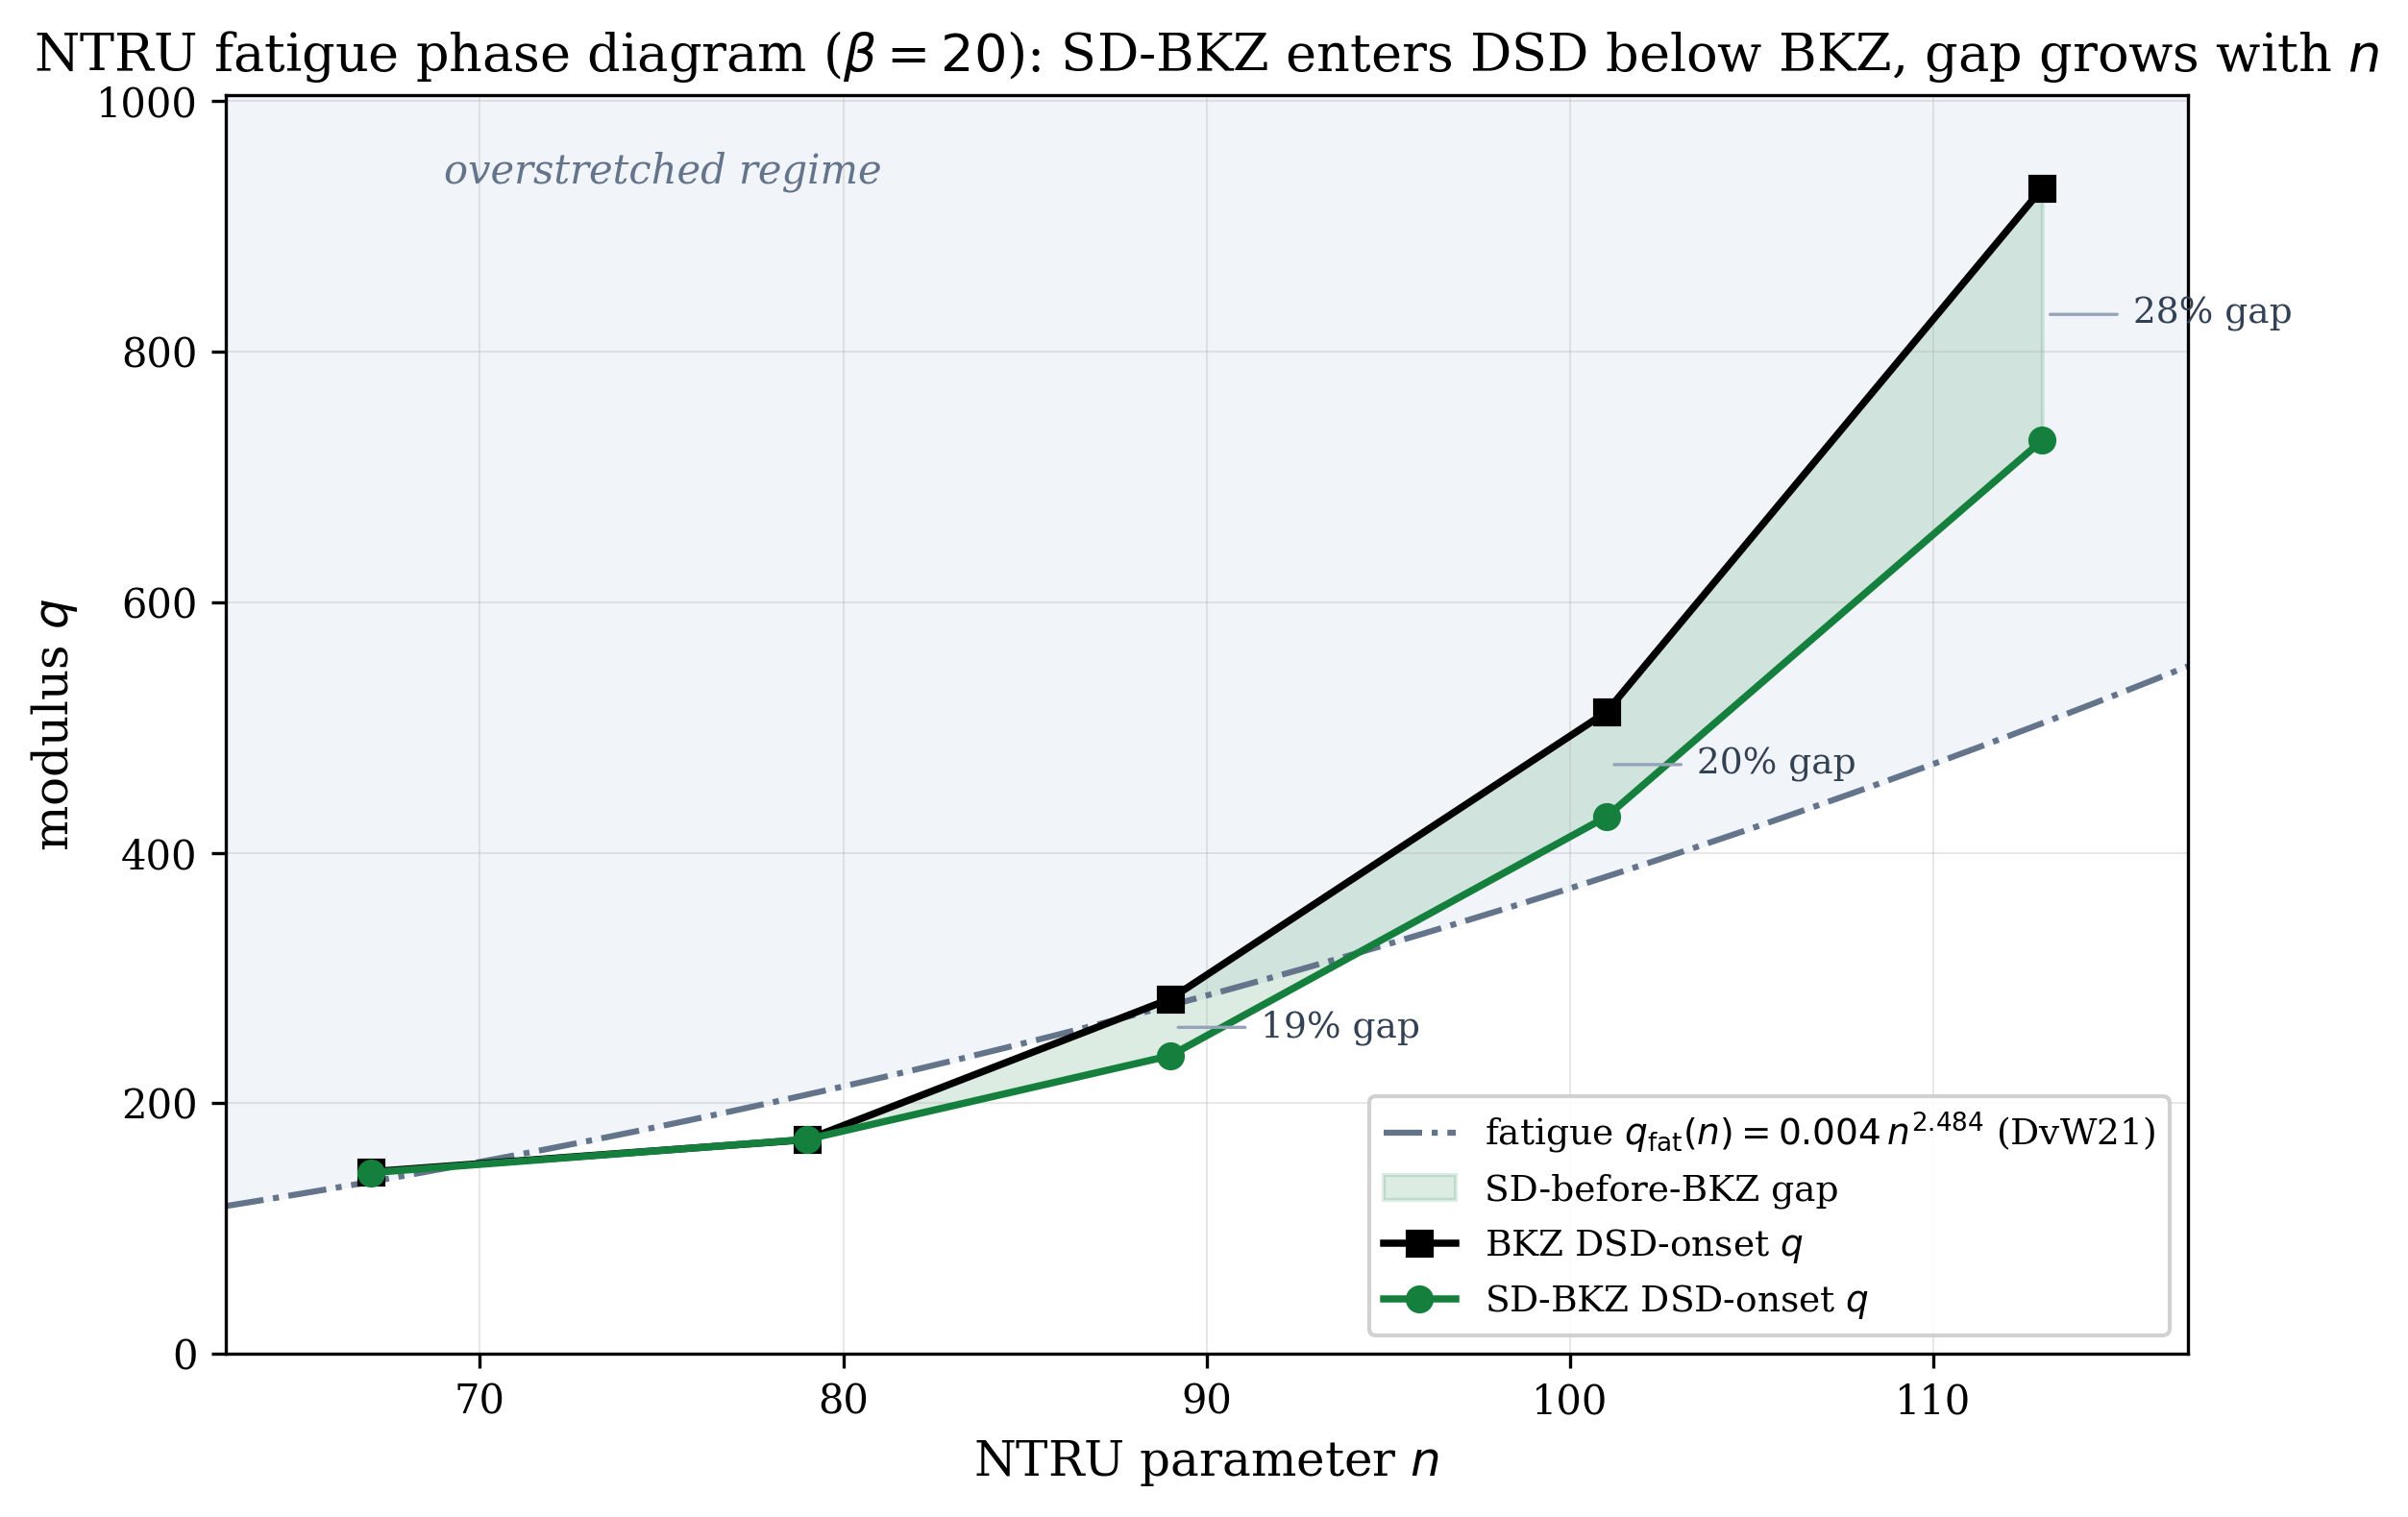
\includegraphics[width=\linewidth]{figs/fatigue_phase}
\caption{NTRU fatigue phase diagram ($\beta=20$). The DvW21 fatigue
curve~\cite{DucasWoerden2021} $q_\mathrm{fat}(n)=0.004\,n^{2.484}$ (an empirical fit) bounds the overstretched
regime (shaded). The measured reference-free DSD-onset curves (two-part
criterion, Table~\ref{tab:dsdgap}) show SD-BKZ entering dense-sublattice
discovery at lower $q$ than BKZ, the gap (band) $19\%$ at $n=89$ and $101$
and $28\%$ at $n=113$ (the $n\le79$ onsets measure the criterion,
Table~\ref{tab:dsdgap}). The onsets cross the fatigue curve rather than lying within the
shaded regime: SD onset$/q_\mathrm{fat}=0.86,1.13,1.45$ at
$n=89,101,113$, i.e.\ below $q_\mathrm{fat}$ at $n=89$ and
increasingly above it from $n=101$, where the $50\%$-rate onset is a stricter
threshold than the asymptotic fit.\label{fig:phase}}
\end{figure}

Figure~\ref{fig:sigmoids} shows the DSD-rate curves from which these onsets
are read.

\begin{figure}[tbp]
\centering
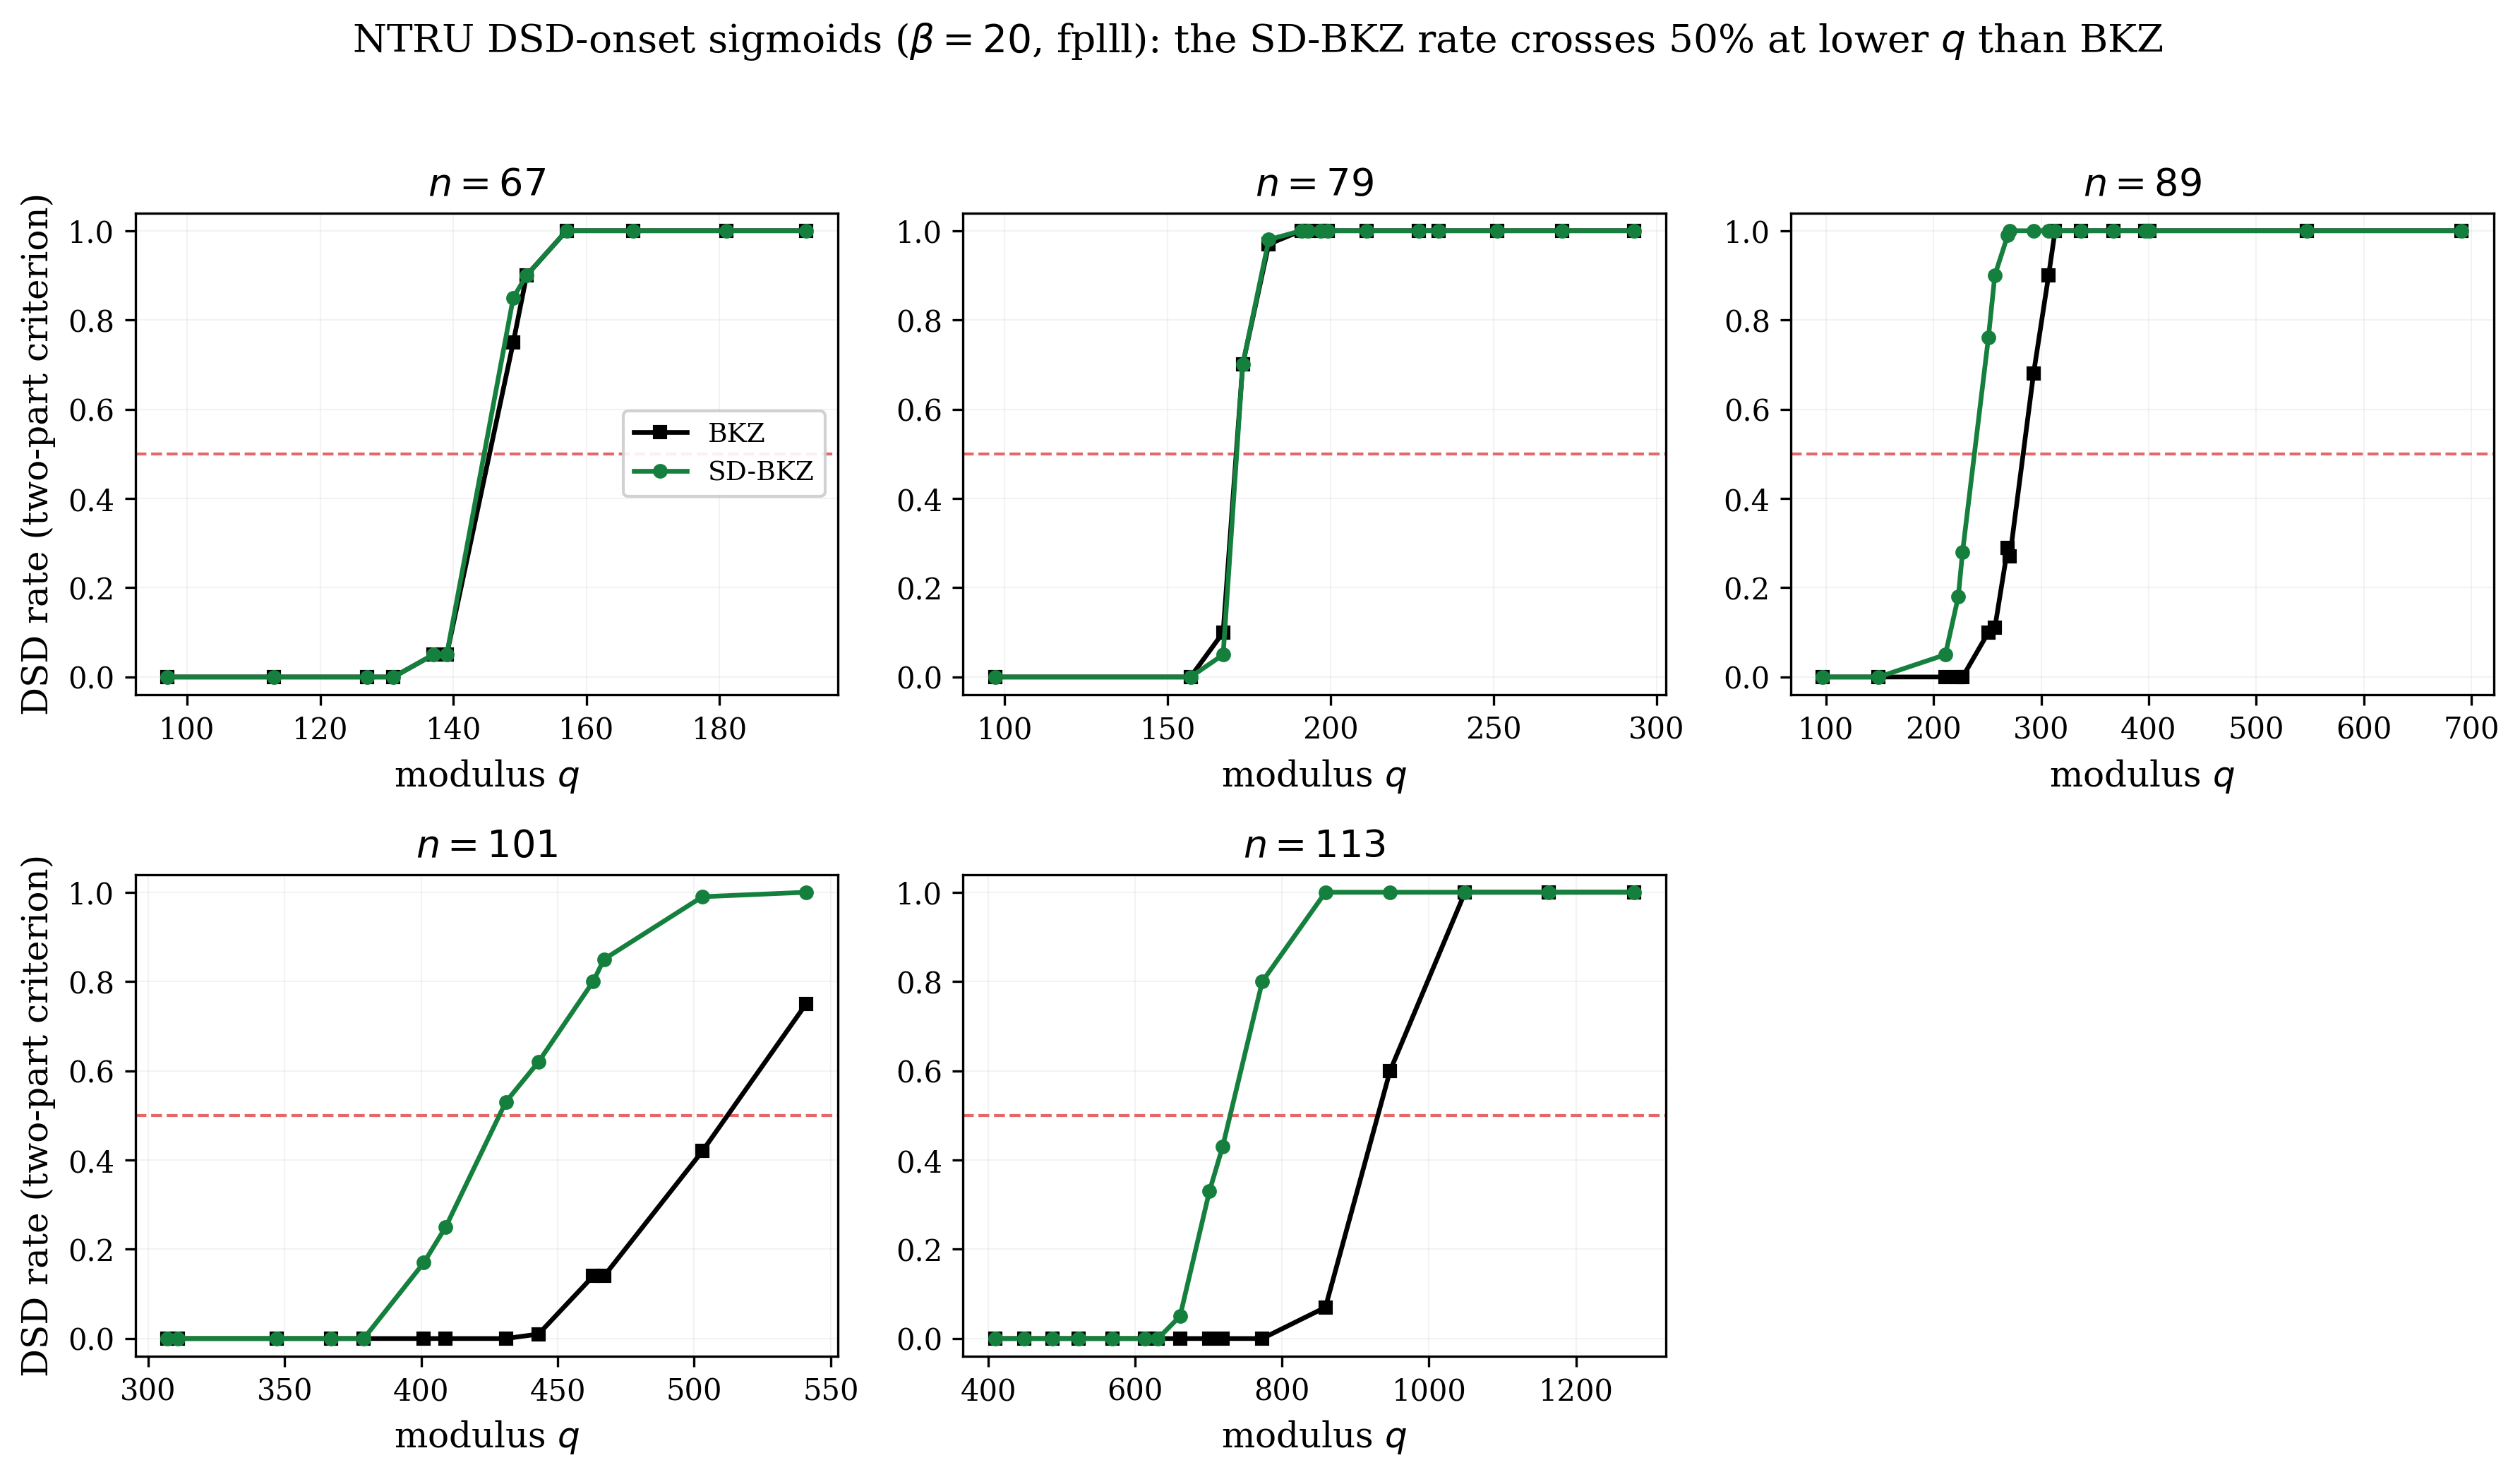
\includegraphics[width=\linewidth]{figs/onset_sigmoids}
\caption{DSD-onset sigmoids ($\beta=20$, fplll, 50 tours): the fraction of seeds
meeting the two-part DSD criterion as a function of $q$, BKZ vs SD-BKZ, faceted
by $n$ (per-cell $N=100$ in the densified band around each onset, $N=20$
elsewhere, $N=28$ at $n=89$, $q=97$: seeds $1$--$20$ at $250$ bits, $1$--$8$ rerun at $500$; otherwise one precision per cell, $250$--$1000$ bits,
Table~\ref{tab:coverage}).
The onsets of Table~\ref{tab:dsdgap} are the $50\%$ crossings; the SD-BKZ curve
(green) crosses left of BKZ (black) at $n\ge89$. A rate
figure---not the signed $d(\mathrm{LN})$---computed with the same two-part
criterion as the onset table, so the two cannot disagree.\label{fig:sigmoids}}
\end{figure}

\subsection{Convergence dynamics}
\label{sec:dynamics}
We track the mean $d(\mathrm{LN})$ each tour at one overstretched
modulus per $n$: $q=307$, $409$, $719$ at $n=89$, $101$, $113$. The $n=89$ cell lies above both $50\%$
onsets of Table~\ref{tab:dsdgap} (DSD rate SD $100\%$ / BKZ $90\%$; $68/100$
BKZ runs stop early on stagnation, median $46$ tours); the other two lie below
both (SD $25\%$ / $43\%$, BKZ $0\%$, every BKZ run at the $50$-tour cap).
Roughly midway through its run SD-BKZ reaches the final $d(\mathrm{LN})$ that
BKZ attains only at the end. Per seed, the first tour at which SD-BKZ drops
below that seed's BKZ final value has median $19$ (interquartile range
$16$--$22$) at $n=89$, $27$ ($26$--$28$) at $n=101$ and $26$ ($25$--$27$) at
$n=113$; $98$, $100$ and $99$ of $100$ seeds cross
(Figure~\ref{fig:crossover}). Tours-to-match is not monotone across the three
cells, which straddle the onset, so no dimension trend is claimed.

\begin{figure}[tbp]
\centering
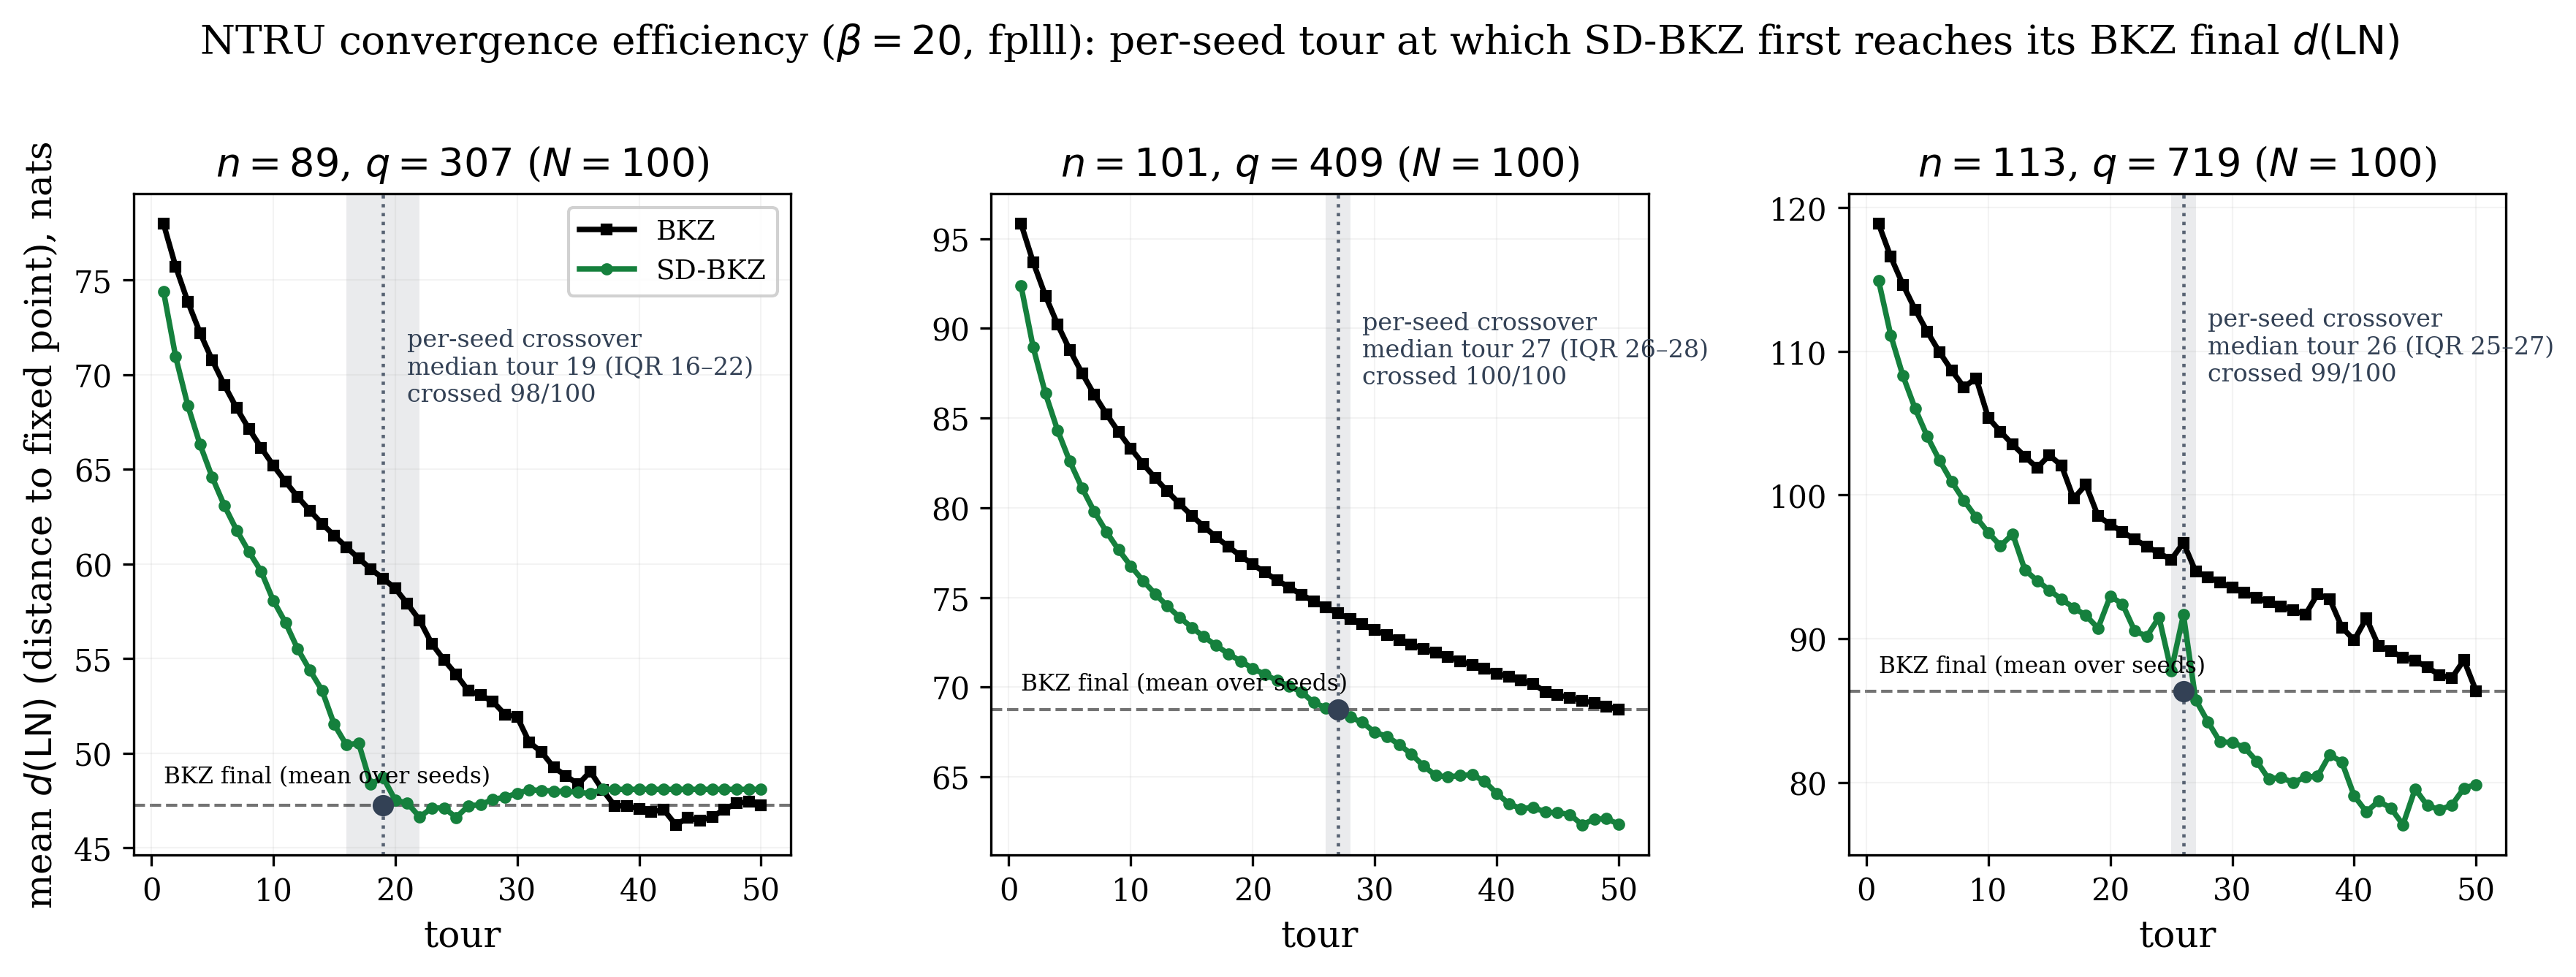
\includegraphics[width=\linewidth]{figs/crossover_dynamics}
\caption{NTRU convergence dynamics ($\beta=20$, fplll, $N=100$ per cell): mean
per-tour $d(\mathrm{LN})$ for BKZ and SD-BKZ at one overstretched $q$ per $n$
($q=307,409,719$ at $n=89,101,113$, i.e.\ $1.10$, $1.07$, $1.43\times
q_\mathrm{fat}$; at $n=101$ and $113$ these sit just below the $50\%$ SD onsets
of Table~\ref{tab:dsdgap}, $428.6$ and $729.2$); each seed is carried forward
at its own final value after its run
stops, so the curves end at the per-seed final means. Dashed: BKZ final value
(mean over seeds). Marked: median per-seed crossover tour, shaded
interquartile range, and the number of seeds that cross (the rest are
censored). The median crossover tour is $19$, $27$, $26$ ($q=307$, $409$,
$719$)---not monotone across these cells, which straddle the onset of
Table~\ref{tab:dsdgap}. The
absolute $d(\mathrm{LN})$ heights are reference-dependent; the reported result is
the crossover \emph{tour} (timing against BKZ's own converged value), not the
curve heights or their end-of-run gap.\label{fig:crossover}}
\end{figure}

Figure~\ref{fig:phasemap} summarises the explored $(n,q)$ plane.

\begin{figure}[tbp]
\centering
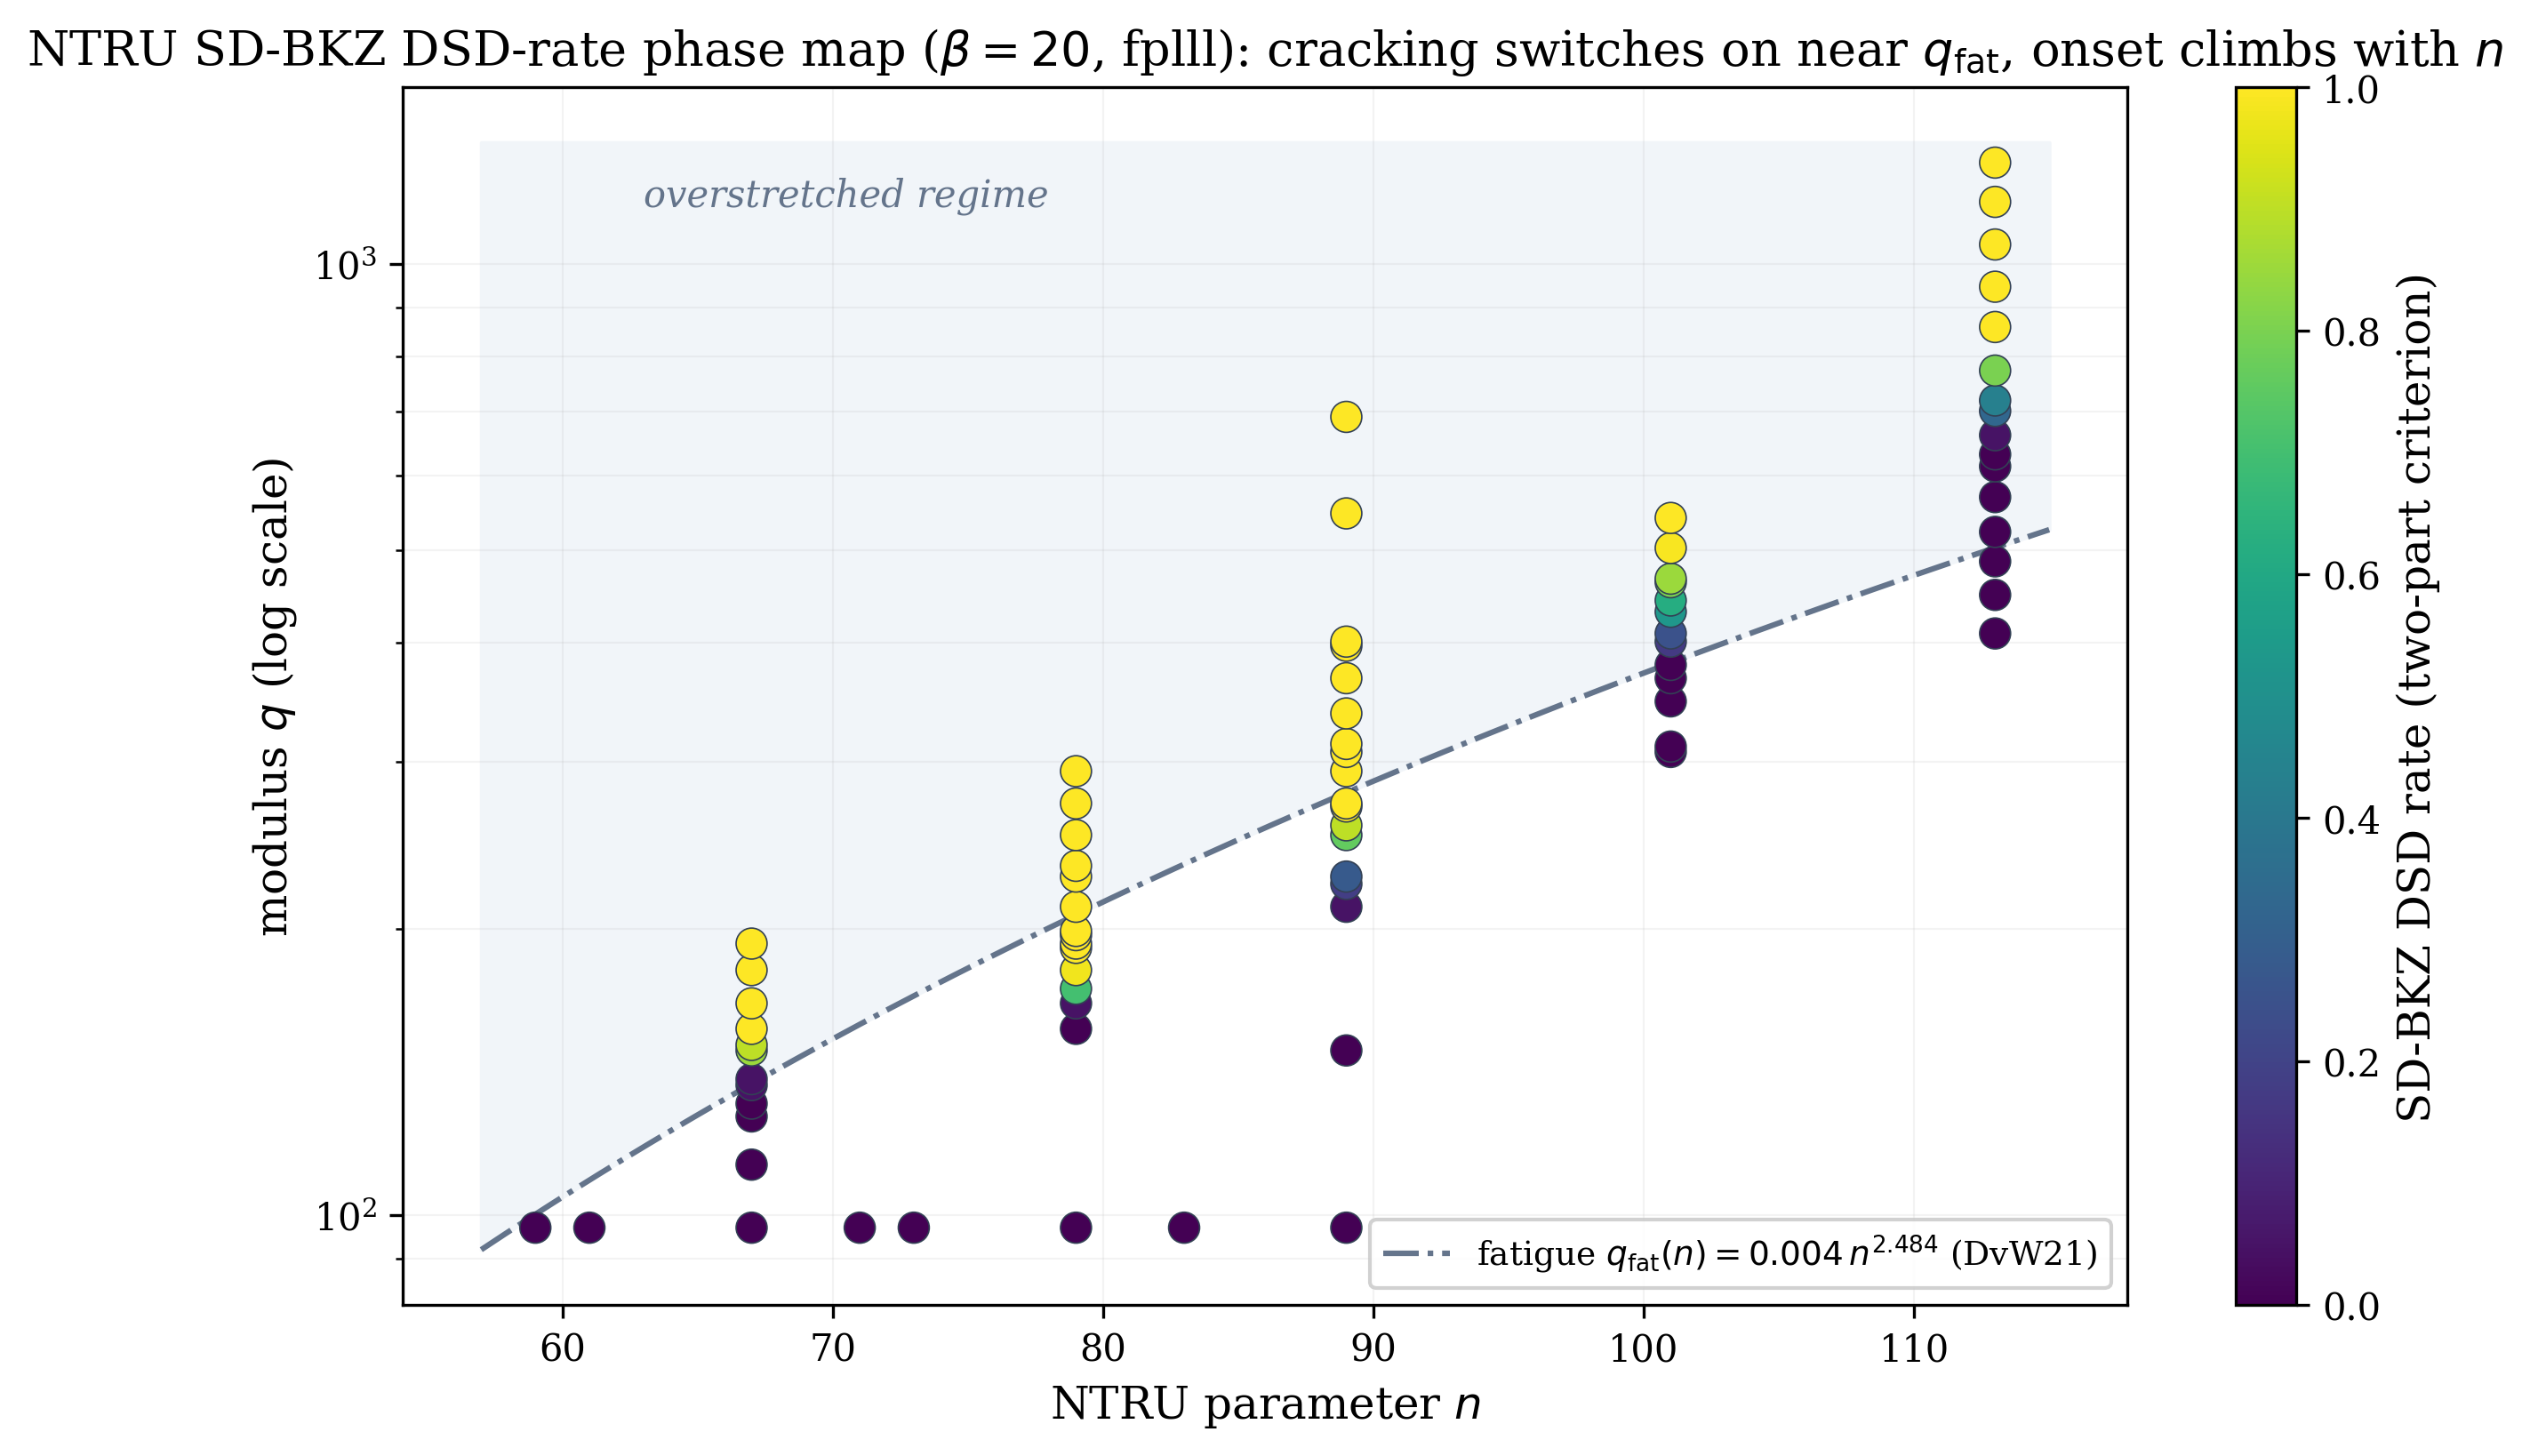
\includegraphics[width=\linewidth]{figs/phase_map}
\caption{SD-BKZ DSD-rate phase map over the $(n,q)$ plane ($\beta=20$, fplll):
colour is the SD-BKZ DSD rate (two-part criterion) at each measured cell, with
$q_\mathrm{fat}(n)$ overlaid. DSD switches on near the fatigue curve
(below it at $n=89$, above it from $n=101$) and the onset modulus climbs
with $n$; $n=127$ is not drawn (Section~\ref{sec:fatigue}). The grid is irregular---a full $q$-ladder at
some $n$, a single $q=97$ point at others---so it is drawn as a scatter; the gaps
are coverage, not interpolation.\label{fig:phasemap}}
\end{figure}

\section{Cross-Engine: SD-BKZ on a Sieve Oracle}
\label{sec:xengine}

\paragraph{The Hermite factor is uninformative where $\mathbf b_1$ stays a $q$-vector and diverges where it does not.}
At $q=97$, $\beta=40$, $n=101/113$, neither variant on either engine
displaces the leading $q$-vector ($20/20$ seeds per cell), so the Hermite
factor $\|\mathbf b_1\|/\det^{1/d}=\sqrt q\approx9.85$ agrees by
construction: bit-identical on G6K, and on fplll differing only by
log-determinant drift ($|\Delta\mathrm{HF}|\sim10^{-6}$, outliers to
$1.8\times10^{-5}$). $d(\mathrm{LN})$ separates the variants on every seed,
SD lower by a median $+1.19/+1.46$ nats on fplll and $+1.34/+1.60$ on G6K.
At $n=67$ both variants end on the same short vector ($20/20$ seeds, both
engines) and $d(\mathrm{LN})$ differs by $<0.08$ nats. At $n=89$ ($q=97$,
$100$ seeds), $\mathbf b_1$ is displaced (identical on $0/100$ seeds;
$|\Delta\mathrm{HF}|$ median $0.24$ fplll, $0.45$ G6K), so the Hermite factor
diverges on every seed, fired or not. The $n=101/113$ pattern is consistent
with RHF-equality under a non-exact oracle~\cite{ABLR21,Rowell2024}.

\paragraph{Cross-engine validation of the construction.}
A fplll-vs-G6K comparison at $q=97$ ($n=89/101/113$, 20 seeds each,
$\beta=40$, 50 tours) confirms the self-dual G6K construction of
Section~\ref{sec:setup-engines} is sound (Table~\ref{tab:xeng-sound}). A run ``fires'' when its first GS log-norm
drops below $3.5$, a loose screen used only for this check, never as a DSD
flag.

\begin{table}[tbp]
\centering
\caption{Cross-engine soundness at $q=97$ (fired $=$ first GS log-norm $<3.5$, agreement screen only): fplll never fires where G6K does not; the jointly-fired $n=89$ seed matches exactly ($2.332$), and the single G6K-only fire is the sieve finding a vector enumeration misses. Jaccard $1.00$ rows are vacuous ($0/0$).\label{tab:xeng-sound}}
\begin{tabular}{rccc}
\toprule
$n$ & G6K fired & fplll fired & Jaccard \\
\midrule
89  & 2/20 & 1/20 & 0.50 \\
101 & 0/20 & 0/20 & 1.00 \\
113 & 0/20 & 0/20 & 1.00 \\
\bottomrule
\end{tabular}
\end{table}

\paragraph{At a matched $\beta=40$, $n=89$, both engines put the SD-vs-BKZ DSD-onset gap under $0.5\%$ of $q$.}
We run the \emph{same} grid (15 moduli $q\in[97,211]$, dense onset window
$q\in\{191,193,197,199\}$) on both engines under the two-part DSD criterion of
Section~\ref{sec:bg-obs}. The G6K sweep adds four $N=20$ saturation cells
$q\in\{257,307,401,521\}$ ($100\%$ DSD on both legs, 500-bit precision at
$q\ge401$), counted in Table~\ref{tab:coverage}. The $b_1>1.5$ test alone
over-fires on uniformly-reduced sub-fatigue bases, where the tail is cleared
but the profile has not collapsed: read as a DSD flag, it turns the $q=137$
clearing counts of Table~\ref{tab:g6konset} into a spurious cross-engine DSD
gap.

Under the two-part criterion the gap nearly vanishes: at $q=137$ neither
variant fires DSD on either engine, and the dense window pins the onset
(Table~\ref{tab:g6konset}). The fplll gap is $+0.16$ modulus units (95\% CI
$[-0.06, +0.49]$; all CIs here are deterministic per-cell bootstraps,
$B=10^{4}$) and the G6K gap $+0.82$ ($[+0.27, +3.17]$): $0.08\%$ and
$0.42\%$ of $q$, though G6K's interval excludes zero. The long G6K right tail
is a near-crossing effect: the G6K SD onset sits ${\approx}0.14$ above the
$q=193$ cell, whose rate $0.49$ is one seed short of the crossing, leaving a
slight SD$<$BKZ tendency on the sieve. The DSD rate rises smoothly through the
window ($37\%$ at $q=191$ to $85\%$ at $q=199$, $100\%$ at $q=211$,
near-identical for both variants and engines), and densifying from $N=40$ to
$N=100$ moved every onset by less than one modulus unit, so the near-zero gap is
measurement-resolved.

\begin{table}[tbp]
\centering
\caption{Cross-engine at $n=89$, $\beta=40$, $50$ tours, under the proper two-part DSD criterion: both
engines reach DSD-onset together (${\approx}q=194$, dense onset window, 100
seeds/cell) with an SD-vs-BKZ gap under $0.5\%$ of $q$ (G6K's $95\%$ interval excludes zero). The separate min-GS-clearing event ($\min_i\log\|\mathbf{b}_i^\ast\|>1.5$
alone: aggressive tail reduction, \emph{not} DSD) shows SD$>$BKZ on both engines
and a sieve-vs-enum structural difference ($q=137$, 100 seeds).\label{tab:g6konset}}
\begin{tabular}{lcccc}
\toprule
 & \multicolumn{2}{c}{fplll (enum)} & \multicolumn{2}{c}{G6K (sieve)} \\
\cmidrule(lr){2-3}\cmidrule(lr){4-5}
 & SD & BKZ & SD & BKZ \\
\midrule
two-part DSD @ $q{=}137$            & 0/100 & 0/100 & 0/100 & 0/100 \\
two-part DSD-onset ($50\%$-rate)    & 193.7 & 193.8 & 193.1 & 194.0 \\
\midrule
min-GS-clearing @ $q{=}137$         & 38/100 & 12/100 & 61/100 & 23/100 \\
median $\min_i\log\|\mathbf{b}_i^\ast\|$ & 0.255 & 0.104 & \textbf{1.844} & 0.140 \\
\bottomrule
\end{tabular}
\end{table}

\paragraph{Where the tail clearing lands: a cross-engine per-position view.}
The min-GS-clearing event of Table~\ref{tab:g6konset} redistributes profile
mass rather than improving it uniformly (Figure~\ref{fig:perpos}). The
pattern holds on both engines, the sieve slightly larger in magnitude.

\begin{figure}[tbp]
\centering
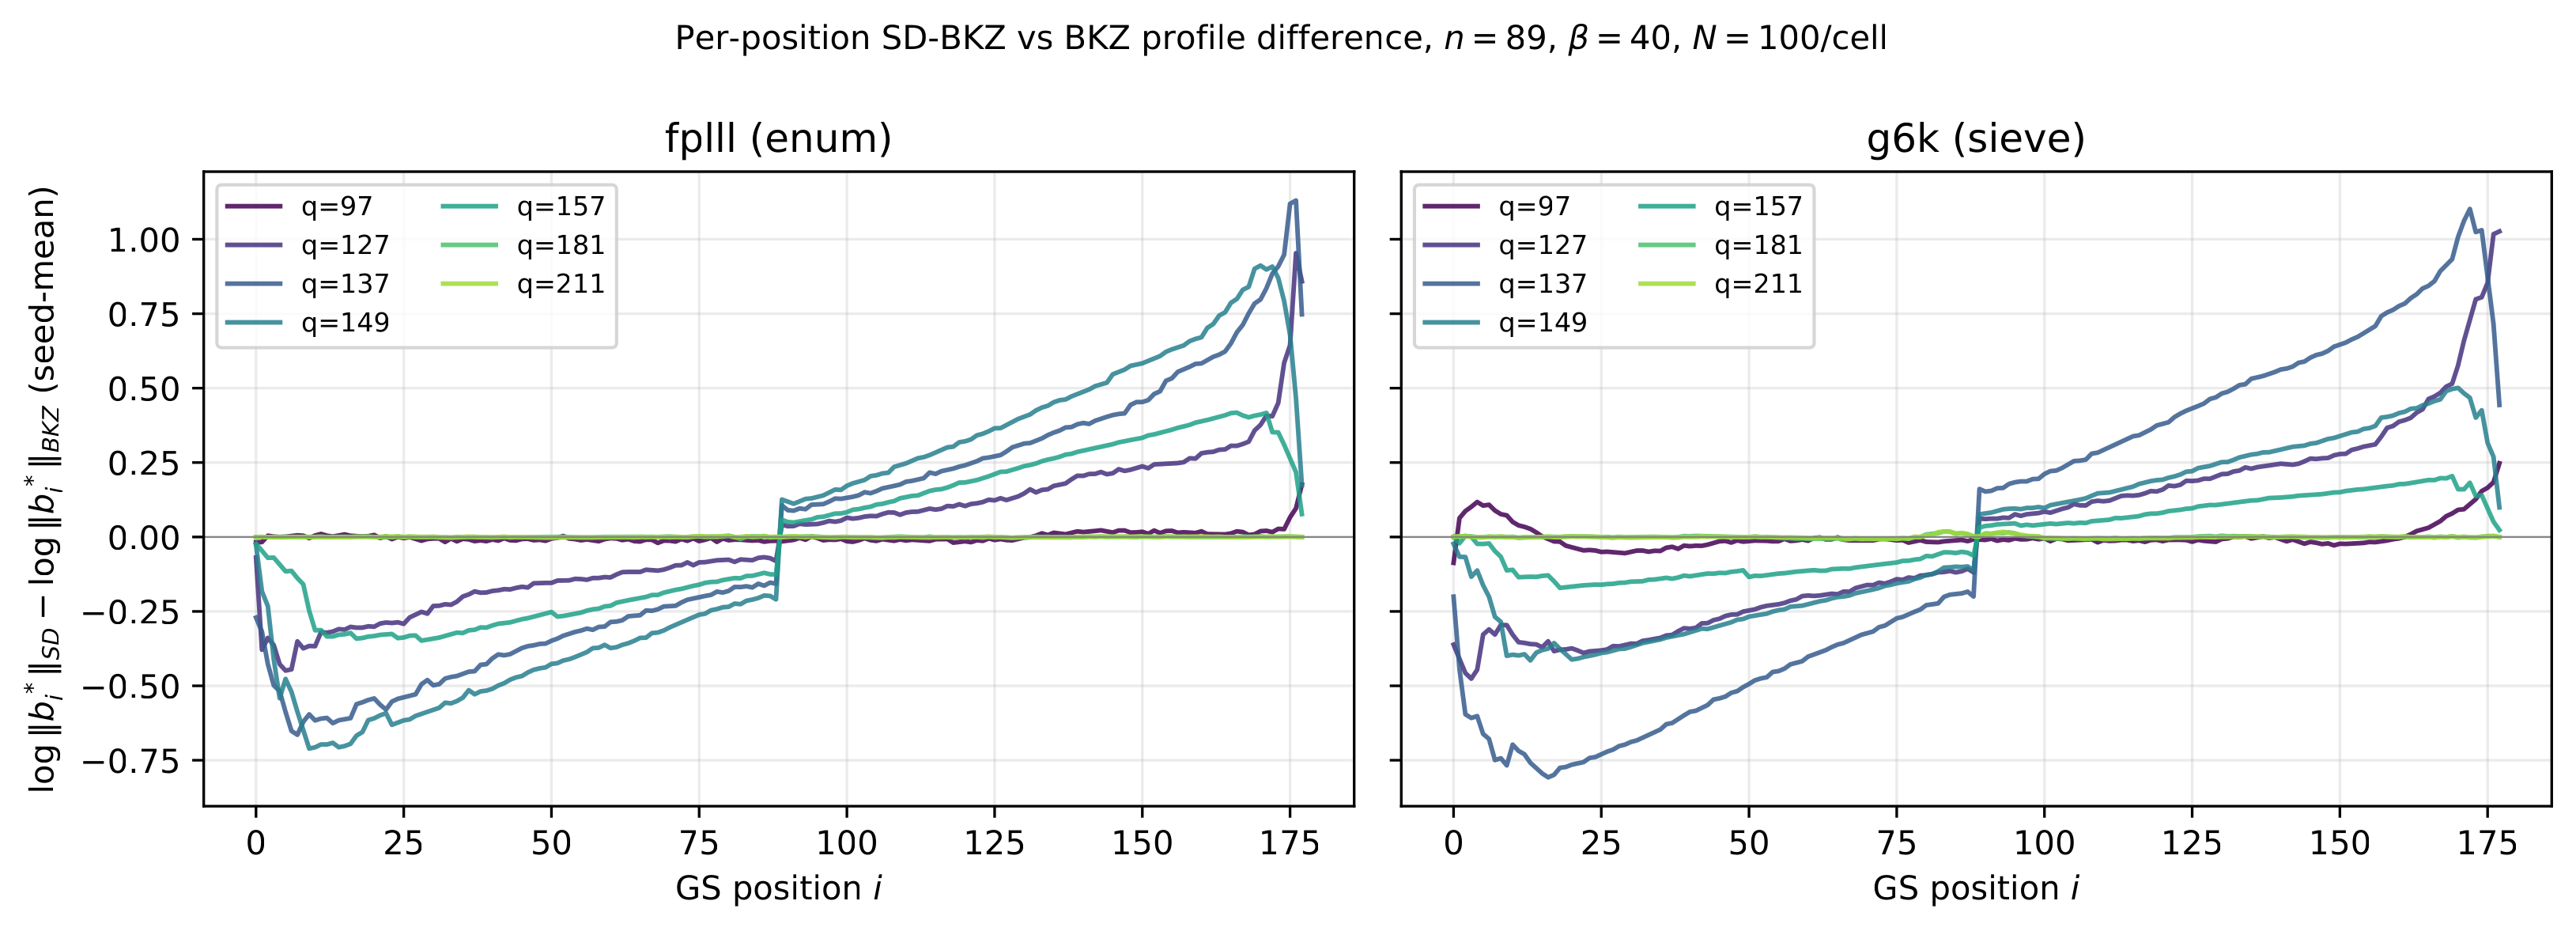
\includegraphics[width=\linewidth]{figs/per_position_attribution}
\caption{Per-position profile difference
$\log\|\mathbf{b}_i^\ast\|_{\mathrm{SD}}-\log\|\mathbf{b}_i^\ast\|_{\mathrm{BKZ}}$
at $n=89$, $\beta=40$ (100 seeds/cell) over a $q$-sweep, for the fplll
enumeration (left) and G6K sieve (right) engines. Self-dual reduction
redistributes mass head-down/tail-up in the pre-onset band ($q\in[127,157]$),
peaking in the last few GS vectors, and is flat at $q\ge181$; both engines
agree. (The step at GS position $i=n$ is the $q$-vector-head / reduced-tail
boundary, not an artefact.) The redistribution is ${\approx}95\%$ predicted by slope flattening
alone ($R^2\approx0.95$), so it visualises the flattening rather than a distinct
mechanism.\label{fig:perpos}}
\end{figure}

At $\beta=40$, $n=89$ therefore does not reproduce the $\beta=20$ DSD-onset
gap of Section~\ref{sec:fatigue}.

At $n=101$ and $n=113$ the picture changes (Table~\ref{tab:xengdim},
Figure~\ref{fig:xengonset}). At $n=101$ a coarse $q$-grid ($50$ tours,
$250$-bit precision; fplll 14 primes $q\in\{127,\dots,463\}$ plus $q=97$,
G6K the three bracketing primes $q\in\{241,271,307\}$ plus $q=97$) recovers a $9\%$ SD$<$BKZ DSD-onset
gap on fplll (per-cell bootstrap over the 14 $N=40$ cells, $95\%$ CI
$[6.1\%,11.1\%]$) and $7\%$ on G6K, where both onsets interpolate within the
single interval $(241,271)$ and no interval is reported. At the transition
cell $q=271$ each engine's SD-BKZ fire set is a near-superset of its BKZ set
on byte-identical bases; the G6K zero-cell split is also significant under an
exact two-sided sign test ($p\approx1.5\times10^{-5}$). At $n=113$ the
extended $q$-grid \emph{locates} the onset on both oracles ($7\%$ gap fplll,
$6\%$ G6K), and at $q=487$ SD-BKZ fires on a strict superset of BKZ's seeds
on both (sign test $p\approx3.8\times10^{-6}$ and $1.2\times10^{-4}$). All
four onsets lie below the fatigue estimate $q_{\mathrm{fat}}(113)\approx503$,
by $1\%$ (fplll BKZ) to $9\%$ (G6K SD).

\begin{table}[tbp]
\centering
\caption{Cross-engine DSD-onset beyond $n=89$ ($\beta=40$, $N=40$ seeds/cell
except $q=97$ at $N=20$; fplll 15-cell and G6K 4-cell $q$-grids at $n=101$,
two-part criterion). The gap is established on \emph{both} engines at $n=101$ and
$n=113$ (the extended $q$-grid $\{487,\dots,859\}$ locates the $n=113$ onset). The
$n=89$ matched-$\beta$ result is Table~\ref{tab:g6konset}.\label{tab:xengdim}}
\begin{tabular}{llccl}
\toprule
$n$ & engine & SD onset & BKZ onset & transition cell (SD vs BKZ fire) \\
\midrule
101 & fplll & 257.3 & 280.7 & $q{=}271$: $36/40$ vs $13/40$ ($24{:}1$, $\chi^2{=}21.2$) \\
101 & G6K   & 249.9 & 268.3 & $q{=}271$: $39/40$ vs $22/40$ ($17{:}0$, $\chi^2{=}17.0$) \\
113 & fplll & 464.6 & 499.0 & $q{=}487$: $34/40$ vs $15/40$ ($19{:}0$, $\chi^2{=}19.0$) \\
113 & G6K   & 456.3 & 482.2 & $q{=}487$: $36/40$ vs $22/40$ ($14{:}0$, $\chi^2{=}14.0$) \\
\bottomrule
\end{tabular}
\end{table}

\begin{figure}[tbp]
\centering
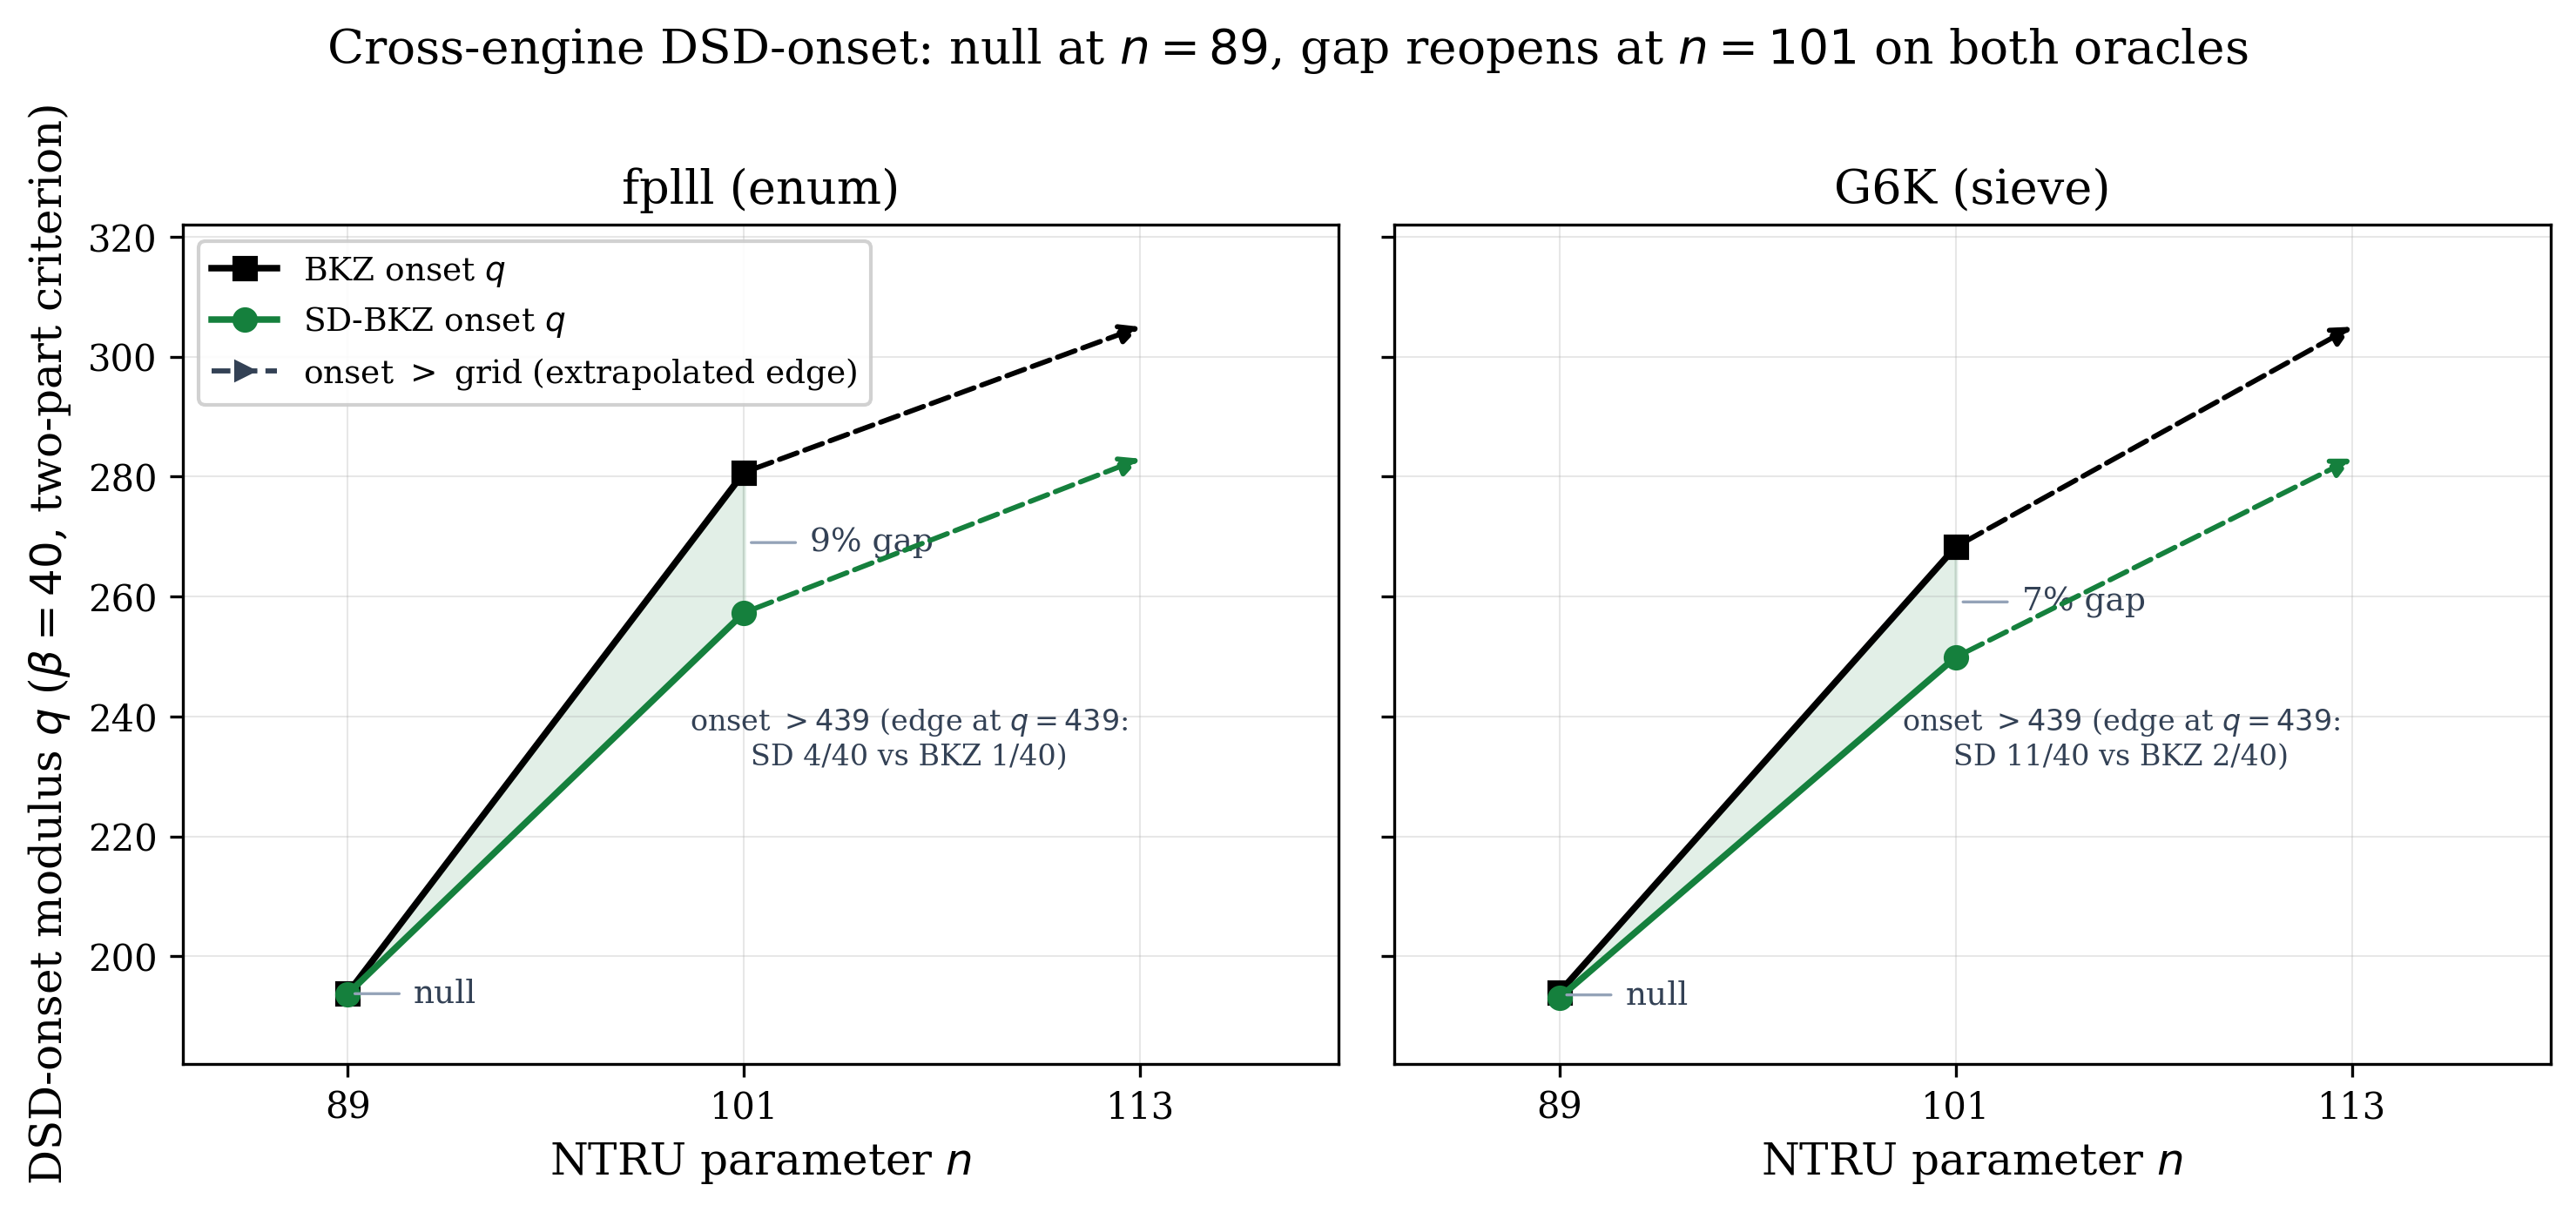
\includegraphics[width=\linewidth]{figs/xengine_onset}
\caption{Cross-engine reference-free DSD-onset $q$ vs $n$ at $\beta=40$
(two-part criterion), faceted by oracle (fplll enumeration, left; G6K sieve,
right). A gap under $0.5\%$ at $n=89$ (SD${\approx}$BKZ${\approx}q{=}194$, dense
window, 100 seeds/cell); the SD$<$BKZ gap reopens at $n=101$ ($9\%$ fplll, $7\%$
G6K) and persists at $n=113$ ($7\%$ fplll, $6\%$ G6K), $N=40$/cell. The extended
$q$-grid $\{487,\dots,859\}$ locates the $n=113$ onset. Mirrors Tables~\ref{tab:g6konset}
and~\ref{tab:xengdim}.\label{fig:xengonset}}
\end{figure}

The matched-$\beta$ comparison does surface a structural difference between
the oracles. The min-GS-clearing event fires more often under SD-BKZ
than BKZ on both engines (Table~\ref{tab:g6konset}). Under SD-BKZ the median
$\min_i\log\|\mathbf{b}_i^\ast\|$ is $1.59$ nats higher on the sieve
(${\approx}4.9\times$ in norm) because the sieve clears $61/100$ seeds
against enumeration's $38/100$; paired per seed, the median ratio is
$1.10\times$. Under plain BKZ the difference is small. Both engines start from the byte-identical
primal basis ($100/100$ seeds) with the determinant conserved (median drift
${\sim}10^{-6}$).

Where the min-GS-clearing event fires, the \emph{signed} $d(\mathrm{LN})$
advantage is large and negative on both engines, because an aggressively
reduced $q$-ary tail is far from the LWE-derived reference.

\section{The Frontier: \texorpdfstring{$n\ge157$}{n>=157} on the Sieve}
\label{sec:frontier}

Of the fplll cells here, $25$ ($500$ seeds: every $n=157$ and $n=181$
cell, three each at $n=167$ and $173$) were measured with the double-precision
GSO and carry $r_{ii}\le0$ floors (Appendix~\ref{sec:p1corr}); the other
fplll cells were measured in MPFR, and they and the G6K final profiles
conserve $\log\det$ to $4\times10^{-10}$. The flag reduces to its $b_1$
floor at these dimensions (Section~\ref{sec:bg-obs}). Every result here is scored by
\texttt{secret\_exact\_match} (Section~\ref{sec:bg-obs}), onset being its
$50\%$ crossing per variant; the $12$ all-ones legs that
\texttt{secret\_recovered} would add are excluded. $\beta\ge50$ exceeds fplll's enumeration reach
here, so those cells run on G6K~\cite{G6K2019}. Table~\ref{tab:frontier}
summarises this corpus, separate from Table~\ref{tab:coverage}.

\begin{table}[tbp]
\centering
\caption{Frontier recovery ladders, $50$ tours ($\dagger$: $580$; $\ddagger$:
G6K build that rejects an overflowing sieve reduction). The $q$
range is in units of $q_\mathrm{fat}(n)=0.004\,n^{2.484}$ with the number of
$q$ cells in parentheses; $N$ is seeds per cell; SD-BKZ and BKZ give
\texttt{secret\_exact\_match} legs pooled over the ladder, with the peak per-cell
rate or the $50\%$-crossing onset; p.\ marks pooled entries from cells under
$20$ seeds (per-cell entries carry their $N$), c.\ seeds
right-censored at the wall cap, -- a rung with no completed seed.\label{tab:frontier}}
\scriptsize
\setlength{\tabcolsep}{2pt}
\begin{tabular}{rrlllll}
\toprule
$n$ & $\beta$ & engine & $q/q_\mathrm{fat}$ & $N$ & SD-BKZ & BKZ \\
\midrule
157 & 40 & fplll & 0.97--3.07 (13) & 20 & onset $2.07\times$, to $100\%$ & onset $2.40\times$, to $85\%$ \\
163 & 40 & fplll & 2.00--3.85 (18) & 20--100 & onset $2.47\times$, peak $75\%$ & none, peak $40\%$ \\
167 & 40 & fplll & 2.00--4.97 (28) & 20 & $116/560$, peak $40\%$ & $49/560$, peak $20\%$ \\
167 & 40 & fplll$^\dagger$ & 2.30 (1) & 8 & $7/8$ (p.) & $6/8$ (p.) \\
167 & 40 & G6K & 2.38 (1) & 80 & $9/80$ & $2/80$ \\
173 & 40 & fplll & 2.20--4.95 (14) & 20 & $7/280$, peak $10\%$ & $4/280$, peak $5\%$ \\
173 & 40 & G6K & 2.81 (1) & 80 & $3/80$ & $1/80$ \\
179 & 40 & fplll & 2.00--3.22 (5) & 20 & $0/100$ & $0/100$ \\
179 & 40 & G6K & 2.91 (1) & 80 & $0/80$ & $0/80$ \\
179 & 40 & G6K$^\dagger$ & 2.91 (1) & 20 & $6/20$ & $1/20$ \\
181 & 40 & fplll & 1.90--3.62 (6) & 20 & $0/120$ & $0/120$ \\
\midrule
179 & 50 & G6K & 2.00--3.22 (5) & 20 & onset $2.54\times$, $33/100$ & $17/100$, peak $30\%$ \\
181 & 50 & G6K & 1.60--4.00 (9) & 20 & $41/180$, plateau $35$--$50\%$ & $17/180$, peak $25\%$ \\
183 & 50 & G6K & 2.75 (1) & 6 & $1/6$ (p.) & $0/6$ (p.) \\
185 & 50 & G6K & 2.68--3.79 (3) & 6--8 & $2/21$ (p., 1 c.) & $1/21$ (p., 1 c.) \\
\midrule
179 & 60 & G6K & 2.00 (1) & 6 & $6/6$ (p.) & $6/6$ (p.) \\
179 & 60 & G6K$^\ddagger$ & 2.00 (1) & 6 & $6/6$ (p.) & $6/6$ (p.) \\
181 & 60 & G6K & 1.36--2.83 (4) & 4--20 & $0/4$, $3/20$, $4/4$, $5/5$; onset $1.78\times$ & $0/4$, $1/20$, $4/4$, $5/5$; onset $1.80\times$ \\
181 & 60 & G6K$^\ddagger$ & 1.36--2.83 (4) & 4--20 & $0/4$, $3/20$, $4/4$, $5/5$; onset $1.78\times$ & $0/4$, $1/20$, $4/4$, $5/5$; onset $1.80\times$ \\
185 & 60 & G6K & 1.85--3.79 (4) & 4--20 (8 c.) & $0/4$, $18/18$, $2/2$, --; onset $2.06\times$ & $0/4$, $15/18$, $2/2$, --; onset $2.11\times$ \\
185 & 60 & G6K$^\ddagger$ & 1.85--3.79 (4) & 4--20 & $0/4$, $20/20$, $4/4$, $4/4$; onset $2.06\times$ & $0/4$, $19/20$, $4/4$, $4/4$; onset $2.08\times$ \\
\bottomrule
\end{tabular}
\end{table}

\paragraph{The clean-onset regime ends between $n=157$ and $163$.}
At $n=157$ both variants cross $50\%$; SD-BKZ reaches $100\%$ ($90\%$ at the grid edge), BKZ $85\%$ at the grid edge. At $n=163$ SD-BKZ
crosses (bracket $[3011,3137]$) but neither saturates: above the crossing
SD-BKZ recovers $147/260$ legs, BKZ $72/260$ (seeds $1$--$20$), and BKZ
never crosses: its $10/20$ at $q=4049$ is $40/100$ over $100$ seeds. Above $n=163$ neither crosses. The $\beta=40$ SD-BKZ onset thus
rises from $0.7$--$0.9\times q_\mathrm{fat}$ at $n=101/113$
(flag-scored, Section~\ref{sec:xengine}) through $1.30$--$1.84\times$ at $n=131$--$151$
(exact-match onsets of the auxiliary ladders, not tabulated) to $2.07\times$ and $2.47\times$ at $n=157$ and
$163$.

\paragraph{The $\beta=40$, $50$-tour recovery wall is a budget, not a dimension.}
Both levers of the $(\beta,\text{tours})$ budget move it: at $n=167$,
$2.30\times$, $580$ tours turn $0/20$ into $7/8$ and $6/8$; at $n=179$ on
G6K, $2.91\times$, they turn $0/80$ into $6/20$ and $1/20$; at $n=181$,
where $\beta=40$ is $0/120$, $\beta=50$ first recovers at $2.30\times$, and
$\beta=60$ crosses at $1.8\times$ ($n=181$) and $2.1\times$ ($n=185$) on both variants and both G6K builds. Every ``wall'' in Table~\ref{tab:frontier} is about
$\beta=40$ at $50$ tours, and the $n=185$ step confounds $+4$ in $n$ with a
lower $q/q_\mathrm{fat}$ at fixed $q$.

\paragraph{SD-BKZ leads per seed; per core-hour the lead thins or reverses.}
Paired on fixed instances, SD-only:BKZ-only is $34$:$1$ at $n=157$ (exact
McNemar $p=2\times10^{-9}$), $134$:$29$ at $n=163$ ($p=2\times10^{-17}$),
$101$:$34$ at $n=167$ ($p=7\times10^{-9}$),
$25$:$9$ at $n=179$ ($p=0.009$) and $34$:$10$ at $n=181$
($p=4\times10^{-4}$, both $\beta=50$); no other cell of
Table~\ref{tab:frontier} reaches two-sided $p<0.05$ (G6K $n=167$: $9$:$2$,
$p=0.065$). The lead extends below recovery. A leg is on the floor when
$\mathbf b_1$ is exactly a $q$-vector (Hermite factor $\sqrt q$). Over $282$
G6K seeds at $50$ tours ($284$ with the reject-build $\beta=60$ cells, same counts; $\beta=40$
at $n=167$, $173$, $179$; $\beta=60$ at $n=181$, $1.36$--$1.66\times$, and
$n=185$, $2.28\times$), no seed has BKZ off the floor with SD-BKZ on it,
against $69$ the other way; with both on the floor SD-BKZ has the lower
$d(\mathrm{LN})$ in $70/70$ ($p\approx2\times10^{-21}$). SD-BKZ costs
$1.6$--$2.6\times$ the core-hours per seed. Per $100$ core-hours it
recovers $7.14$ against $8.41$ at $n=163$ and $3.23$ against $3.49$ at
$n=167$ (fplll $\beta=40$), so on fplll the per-seed lead is not a compute
lead. On G6K $\beta=50$ it recovers $3.31$ against $3.52$ at $n=179$ but
$2.40$ against $1.95$ at $n=181$, so there it is unsettled. At $\beta=60$
it recovers $5.09$ against $7.94$ at $n=179$, $1.82$ against $2.71$ at
$n=181$ and $3.69$ against $5.95$ at $n=185$ on the tolerant build (completed
seeds), and $5.86$ against $9.18$, $1.93$ against $2.88$ and $3.45$ against
$6.25$ on the reject build.

\paragraph{What the sub-$q^2$ basis holds.}
From $2.6\times$ up no $\beta=50$ leg at $n\in\{179,181\}$ remains at the
$q$-vector floor ($0$ of $320$), yet non-recovering legs cluster at squared
norm $9{,}930$--$20{,}068$ whatever $q$ (secret ${\approx}240$). Of the
three shortest rows per leg at $n=179$ ($48$ seeds, $288$ rows), every row
is a $q$-vector or lies in the span of the key's rotations, except $2$ from
one seed at the $2.30\times$ edge (${\approx}0.995\,q^2$): at $2.00\times$
all $48$ rows are $q$-vectors; at $2.91\times$, $\beta=50$ holds
$16$ exact rotations and no $q$-vector, $\beta=40$ $51$ $q$-vectors and no
rotation. The band is the dense sublattice of the key's rotations, found but
not descended: at $\beta=50$ the variants differ in the descent, not
the discovery---dense-sublattice discovery without key recovery, which the flag
of Section~\ref{sec:bg-obs} cannot separate.

\paragraph{Limitations.}
Every count in Table~\ref{tab:frontier} is preliminary against the
$100$-seed standard of Section~\ref{sec:fatigue}. The three $50$-tour G6K
$\beta=40$ cells have fplll mirrors outside the canonical manifest (seeds
$1$--$100$: SD-BKZ $6/100$, $2/100$, $0/100$ against BKZ $0/100$; two-sided
sign test $p=0.008$), not pooled above. Fourteen seeds
of the $n=181$ $\beta=50$ ladder aborted on a per-seed-deterministic G6K
sieve assertion and were rerun on a tolerant build, so the
$2.83$--$4.00\times$ rungs mix two builds. The tolerant build lets a sieve
reduction wrap a $16$-bit coefficient; the $\beta=60$ ladder was rerun on a
build that rejects such a reduction ($\ddagger$). On the tolerant build $8$
seeds at $n=185$ are right-censored at the $48$\,h cap: $q=3907$ seeds $10$
and $16$ repeat one overflowing swap without progress, and the other $6$
($q=4591$, $6491$) complete fewer than $25$ BKZ tours. On the reject build
all $71$ seeds complete; one, cap-killed at $20$ concurrent seeds, was rerun
alone and reproduces the $d(\mathrm{LN})$ it had logged at three tours. Of the $63$ seeds completed on both builds,
$34$ have no rejected reduction and are identical; the other $29$ first diverge
in $d(\mathrm{LN})$ between tours $5$ and $49$, and exact recovery changes on $3$
BKZ legs (all recovered on the reject build) and on no SD-BKZ leg. The table
reports recoveries over completed seeds, with attempted in $N$. On G6K
$61$ of the $69$ seeds with legs in different floor states have a stored
$d(\mathrm{LN})$ advantage below $-100$ nats, so no frontier cell is averaged on stored
$d(\mathrm{LN})$. Twenty concurrent seeds cost $1.8$--$2.2\times$ the
per-seed wall time of four, so wall times are not compared across cells.
Where the DSD flag can be checked against exact recovery, its misses fall
mostly on BKZ legs (SD $10/197$, BKZ $38/169$ at $n=131$--$151$; at $n=127$
a $2.0\%$ flag gap against $0\%$ exact). The flag-scored $\beta=20$ gaps
may therefore overstate the SD-BKZ lead, though the flag-independent
$\mathbf b_1$ rates of Section~\ref{sec:fatigue} ($88/100$ vs $47/100$ at
$n=89$, $q=223$) also favour SD-BKZ.

\section{Discussion}
\label{sec:discussion}
Three observations bear on models that score BKZ variants by RHF alone.
First, the SD-BKZ advantage is \emph{not} a smooth function of dimension
(Section~\ref{sec:dimonset}), so a coarse $n$-grid can miss the
$d(\mathrm{LN})$ spike at $n=71$--$73$, where the DSD flag cannot fire. Second, the
quantity that captures the difference is reference-free
(Sections~\ref{sec:fatigue} and~\ref{sec:frontier}); only the dimension-sweep
spike is reference-robust. Third, an RHF-only model puts both variants' NTRU
DSD-onset at the same modulus. Against an adversary free to pick SD-BKZ over
BKZ at fixed blocksize and tours, it thus misses that BKZ's onset sits
$19$--$28\%$ above SD-BKZ's at $\beta=20$ (Section~\ref{sec:fatigue}) and
$0$--$9\%$ above at $\beta=40$ (Section~\ref{sec:xengine}) on identical
bases ($n=89$--$113$, flag-scored). The gap narrows with $\beta$ at these
matched $n$, and at $\beta=40$ opens only from $n=101$. Every onset here
lies at ${\ge}0.65\,q_\mathrm{fat}$ (flag-scored; exact recovery from
$1.09\,q_\mathrm{fat}$), on $n\le185$ uniform-ternary keys, and moves with
$n$, $\beta$ and tours ($\beta=60$ crosses at $1.8\times$ at $n=181$, where
$\beta=40$ at $50$ tours recovers nothing from $1.9$ to $3.6\times$).
Nothing here is a bit-security estimate, and at the frontier the per-seed lead does not
survive cost normalisation on the fplll ladders (Section~\ref{sec:frontier}).

The move from an RHF-centric view to
sublattice density echoes recursive lattice
reduction~\cite{RecursiveReduction2023}, which complements the Hermite-factor
framing with a Rankin/dense-sublattice one. Ducas and Loyer~\cite{DucasLoyer2025} drive BKZ with a
densest-sublattice ($\mathrm{DSP}_k$) oracle and report no advantage on
generic lattices; our observable is the self-dual variant's dense-sublattice
\emph{onset} on NTRU, a different algorithm and question. Karenin and
Kirshanova~\cite{KareninKirshanova2024} find dense submodules by algebraic
reduction and report that it needs a larger $q$ than classical BKZ; we measure
the classical onset on two oracles. We do not benchmark speed-oriented tools
such as \textsf{flatter}~\cite{RyanHeninger2023}: the object of study is basis
structure at fixed reduction effort, not wall-clock.

The signed
$d(\mathrm{LN})$ is read quantitatively only at $q=97$ and in
Appendix~\ref{sec:kahan}; elsewhere only its sign ($q=137$; the frontier
floor comparison) or crossover tour (Section~\ref{sec:dynamics}) is used. The criterion-sensitivity episode of
Section~\ref{sec:xengine} generalises: a binary structural flag should test
the structure, not a single order statistic that aggressive reduction can
satisfy without it.

\section{Reproducibility}
\label{sec:repro}
Beyond the per-seed JSON / SHA-256 / named-campaign apparatus of
Section~\ref{sec:setup-repro}, the cross-engine soundness records and
DSD-onset tables are committed under
\texttt{results/}\allowbreak\texttt{validation/}, each with its reproduction
recipe (image, campaign, command); the determinism and self-dual-semantics
decisions are recorded in ADRs~005--008. Each figure has one module under
\texttt{analysis/plots/}, regenerated by \texttt{analysis/paper2\_figures.py}:
Figure~\ref{fig:dimonset} from the per-seed \texttt{advantage} field,
Figure~\ref{fig:perpos} from the GS-log-norm profiles,
Figures~\ref{fig:phase}, \ref{fig:sigmoids}, \ref{fig:phasemap}
and~\ref{fig:xengonset} from the two-part DSD criterion
(\texttt{scripts/extract\_dsd\_onset.py}, so figures and onset tables cannot
disagree), and Figure~\ref{fig:crossover} from the per-tour
\texttt{*\_dln\_per\_tour} arrays. The NTRU generator and G6K engine were
added without altering the seed JSON schema, so the companion paper's SHA
baselines are preserved. Every cell of Tables~\ref{tab:coverage}
and~\ref{tab:frontier} regenerates from its named campaign. Code, per-seed
JSON, SHA-256 manifests and \texttt{config/sweep.toml} are in the companion
repository
\url{https://github.com/BrendanChambersBourgeois/sdbkz-benchmark}~\cite{Paper1},
archived under Zenodo concept DOI
\href{https://doi.org/10.5281/zenodo.19686927}{10.5281/zenodo.19686927}.

\section{Conclusion}
\label{sec:conclusion}
BKZ and self-dual BKZ, RHF-equal on LWE-Kannan lattices, also differ on
NTRU: at $\beta=20$ BKZ's dense-sublattice-discovery onset sits $19\%$
above SD-BKZ's in $q$ at $n=89$ and $101$ and $28\%$ at $n=113$
(flag-scored). At matched $\beta=40$ enumeration and
sieving agree on the onset at $n=89$, differ in the sub-fatigue tail, and both
reopen the gap from $n=101$ (Section~\ref{sec:xengine}). At $n\ge157$, in
preliminary cells, the $\beta=40$, $50$-tour wall moves with blocksize and
tours, and SD-BKZ leads per seed but not per core-hour on fplll
(Section~\ref{sec:frontier}). The threat model is an adversary free to pick
SD-BKZ over BKZ at fixed blocksize and tours; the results are toy-size
($n\le185$, $\beta\le60$) and not a bit-security estimate. The
determinism-gated two-engine benchmark is released (Section~\ref{sec:repro}).

\appendix

\section{Corrections to the Companion Paper}
\label{sec:p1corr}

The companion paper~\cite{Paper1} is archived as published. The following
statements are wrong; the values below, recomputed from the per-seed data,
supersede them.

\paragraph{The fplll GSO fix~\cite[\S8]{Paper1}.} The companion paper
attributes the $q=3329$ degeneracy ($38/100$ seeds) to cancellation in
fplll's Gram--Schmidt recurrence and reports that a Kahan-compensated patch
removes it ($0/55$). Both are withdrawn. The reduction ran at $1000$ bits and
is clean; the profiles, $d(\mathrm{LN})$ values and floors come from a
separate double-precision measurement GSO on a $301$-dimensional basis whose
Gram matrix has condition number $2^{55}$--$2^{59}$, beyond $53$-bit
arithmetic. A floor, $\log\|\mathbf b_i^\ast\|=-345.388$, is the value our
code writes when that measurement returns $r_{ii}\le0$. Replaying stored
trajectories bit for bit and measuring the same $64$ bases gives $7$ floors
in double on the stock build, $1$ in double with the corrected patch and none at
$1000$ bits, where the floored positions have
$\log\|\mathbf b_i^\ast\|=0.61$--$1.14$. The $0/55$ was measured at $1000$
bits against a double-measured baseline, on a build whose compensation sign
was inverted. The paired rerun on the corrected build ($14/100$ seeds floored
with compensation, $46/100$ with it zeroed) shows the same effect: the patch
also changes the double-precision measurement.
The counts were also scored differently: $38$ counts a floor in the
\emph{final} profile, $0/55$ any tour; under the any-tour criterion $100$ of
$101$ unpatched seeds show an excursion.
The $n=110$ statement (both algorithms affected in all $22$ seeds) is
also any-tour: $12$ of the $22$ end on the floor, $4$ on both legs.
The median advantage at $n=100$, $+0.57$ to $+0.60$ nats in every arm, is
double-measured; on unfloored tours the double $d(\mathrm{LN})$
error at $n=100$ has median $0.16$ and reaches $1.8$ nats, and the stored
profiles' volume error reaches $2.6$ nats. Measured at $1000$ bits, the
median advantage is $+0.535$ at $n=100$ (100 seeds), $+0.560$ at $n=90$
(30) and $+0.546$ at $n=80$ (50).

\paragraph{The $\beta=40$ peak dimension.} The companion paper states that the
$\beta=40$ advantage peaks at $n=110$ ($1.16$ nats, ``confirmed at 122 seeds'').
At $122$ seeds per cell the $n=100$ mean is $+1.16864$ and the $n=110$ mean
$+1.16313$; the bootstrap $95\%$ interval of the difference is
$[-0.032,+0.043]$, $P(n=100\text{ higher})=0.62$. The peak lies in
$n\in[100,110]$ at ${\approx}1.16$ nats; its dimension is not resolvable at
this sample size.

\paragraph{Loss margin when BKZ wins.} The statement that the mean loss margin
is below $0.04$ nats in every group where BKZ wins any seed is false: of the
$17$ such groups, $11$ exceed $0.04$ nats, reaching $1.452$ nats at $n=140$,
$\beta=40$, where BKZ wins every seed. The sentence holds only in the
coin-flip regime. The quoted SD-BKZ win margin ($0.106$--$1.349$ nats) is
the group mean advantage at $(n,\beta)=(50,40)$ and $(100,30)$; over the
$13$ such groups with SD-BKZ wins it spans $0.061$--$0.417$ nats.

\paragraph{Compute premise of the capability test.} The capability argument
states that BKZ at $3\times$ tours received $14\%$ more compute than SD-BKZ,
extrapolated from the main-sweep runtime table. Measured on the
$400$ capability-test seeds, BKZ at $210$ tours received $8.4\%$ more
wall-clock than SD-BKZ at $70$ tours ($6.5\%$ at $n=50$). The conclusion
(0/400 gaps closed) stands on a smaller handicap.

\paragraph{HF thresholds~\cite[\S4, abstract]{Paper1}.} Outside the outlier
seeds the printed HF differences are measurement error, not differences
between bases. On $3{,}278$ of the $3{,}388$ $q=97$ seeds both variants end
on the same first vector, so their Hermite factors are equal and the true
difference is $0$. The stored values (group means up to $2.2\times10^{-6}$;
$13$ of the $28$ groups without outlier seeds exceed the quoted $10^{-7}$)
are the log-determinant drift of the double-precision measurement, whose
sign sets every RHF ``win'' on those seeds (the companion paper's $42$--$58\%$
win rates). The other $110$ seeds are the outliers below.

\paragraph{Outlier seeds~\cite[\S4.1]{Paper1}.} The starred groups hold $110$ seeds with
$|\Delta\mathrm{HF}|>0.01$, not five; per group, $1$, $31$, $26$, $5$ and
$47$ seeds at $(n,\beta)=(60,20)$, $(70,20)$, $(70,30)$, $(80,30)$, $(80,40)$. Each has one
first vector at $\mathrm{HF}\approx4.65$--$4.67$, on the BKZ side in $64$
seeds and the SD-BKZ side in $46$. All $110$ keep a positive
$d(\mathrm{LN})$ advantage.

\paragraph{Statistics table~\cite[\S4]{Paper1}.} The $t$-test $p$-values are two-sided,
not one-sided as captioned, except $0.008$ at $n=120$, $\beta=40$, which
matches no sidedness (two-sided $0.0070$). The Wilcoxon column mixes two-sided and
one-sided values; its $n=140$, $\beta=30$ entry ($1.5\times10^{-4}$)
reproduces under neither (two-sided $5.8\times10^{-5}$). Of the $24$ groups
at $n=50$--$120$, $23$ are significant for SD-BKZ and $n=120$, $\beta=40$
for BKZ. Shapiro--Wilk is below $0.05$ in two groups ($n=100$, $\beta=20$:
$0.033$; $n=110$, $\beta=40$: $0.049$).

\paragraph{GSO tail hook~\cite[\S5.4, \S8.4]{Paper1}.} At $\beta=30$ the BKZ hook
minimum sits at basis position $355$ of $391$ ($n=130$, $-0.32$ nats) and
$395$ of $451$ ($n=150$, $-0.31$): $36$ and $56$ vectors follow it, more
than $\beta$, so ``fewer than $\beta$ vectors remain'' does not hold there.
The last $33$ and $52$ positions are flat at $\log\|\mathbf b_i^\ast\|\approx0$ in
both algorithms, and the figure's reference lines are anchored over them;
the last five BKZ values lie $0.46$--$0.54$ ($n=130$) and $0.75$--$0.83$
($n=150$) nats above the plotted Li--Nguyen line.

\paragraph{Precision robustness~\cite[\S7.4]{Paper1}.} The $500$-bit rerun at $n=130$,
$\beta=40$ (seeds $1$--$20$) is bit-identical to the $250$-bit main-sweep
seeds $1$--$20$ (mean $-1.282$ in both). The quoted shift from $-1.370$
compared it with seeds $76$--$100$; the $6.4\%$ softening is withdrawn.

\paragraph{Figure captions.} The absolute-$d(\mathrm{LN})$ figure caption quotes
the $\beta=40$ inversion at $n=150$ as SD-BKZ ${\sim}8.4$ vs BKZ ${\sim}6.8$;
those are the $n=140$ values ($8.33$ vs $6.88$). At $n=150$ the means are
SD-BKZ $12.36$ vs BKZ $11.07$; the direction is unchanged. The $q=3329$
degeneracy figure~\cite[\S8]{Paper1} is captioned as $100$ seeds, but its plotting code
loads $101$, pooling the independent seed-101 probe into the block it
validates. The caption counts ($62$ clean, $38$ degenerate) describe
seeds $1$--$100$. The per-position figure puts the $\beta=20$ tail dip
``near position~$0.9$''; from $n=90$ it sits at position $88$--$89$ of the
active block, fractional position $0.97$ ($n=90$) to $0.59$ ($n=150$); at
$n\le80$ there is none.

\section{The \texorpdfstring{$-345$}{-345} Floor on the \texorpdfstring{$n=127$}{n=127} NTRU Cells}
\label{sec:kahan}

Of the $152$ $n=127$ $\beta=20$ seeds (Section~\ref{sec:fatigue}), $16$
carry the measurement floor of Appendix~\ref{sec:p1corr} on $17$ legs in
$10$ cells: each such leg ends with one Gram--Schmidt entry at
$\log\|\mathbf b_i^\ast\|=-345.388$, written when the double-precision
measurement GSO returns $r_{ii}\le0$. It is not a reduction outcome:
$\sum_i\log\|\mathbf b_i^\ast\|=\log\det L$ for every basis, yet each floor
lowers the stored log-determinant by $343.6$--$348.3$ nats. Nor is it a crack:
no floored leg has a $\mathbf b_1$ shorter than squared norm $14{,}187$,
against the key's $175$, and of the $599$ floored legs in the NTRU corpus
that record \texttt{secret\_exact\_match}, none recovers the key.

We reran three of these cells ($q\in\{971,1087,1201\}$, four seeds each;
five floored stock legs, four BKZ and one SD-BKZ) on two patched builds,
one with the compensation sign inverted and one corrected. The floors move:
five on the inverted build (all SD-BKZ, none floored on stock), three on the
corrected build, and no seed floors on the same leg on all three builds.
Four SD-BKZ legs are partial collapses on all three builds ($q=1087$
seed~1, $q=1201$ seeds $1$--$3$; $d(\mathrm{LN})=78$--$85$, determinant
preserved); $\mathbf b_1$ has the key's norm on three of them on the
inverted build, one on stock and none on the corrected build, where no leg
recovers the key. Both patched builds compile fplll with FMA contraction,
which by itself changes the SD-BKZ trajectories, and the patch also changes
the double-precision measurement, so none of these per-leg differences can
be credited to the patch.

\bibliography{abbrev3,crypto,biblio}

\end{document}
